
\newcommand{\kpch}{\ensuremath{h^{-1} \, \text{kpc}}}
\newcommand{\kpc}{\ensuremath{\text{kpc}}}
\newcommand{\solarmh}{\ensuremath{h^{-1} \, M_\odot}}
\newcommand{\solarm}{M_\odot}
\chapter{Forming Vertical Structure in $\Lambda$CDM Discs}\label{ch:paper_iii}
\textbf{This chapter contains a draft of a paper in preparation to be submitted to Monthly Notices of the Royal Astronomical Society. The working title for the paper is ``Vertical Structure and Kicked-Up Stars in $\Lambda$CDM Galaxies". }

\newpage
\section{Abstract}

We present and study vertical structure evolution twelve high resolution simulations of Milky Way stellar discs inserted into cosmological dark matter haloes. The simulations exhibit a wide variety of vertical structure formation arising from bar buckling, interactions with the host halo, and substructure. A systematic study of the effects of the disc's initial dynamical temperature, measured by Toomre $Q$, and the time of insertion on the disc properties is conducted. Inserting a disc into a more equilibrated halo appears to lead to quieter vertical structure evolution, and increasing the disc's internal dynamical temperature appears to have a non-trivial impact. Furthermore, we identify a population of stars that get kicked up to high latitudes in each simulation. Our results are consistent with the idea that a disc-satellite interaction origin of these structures requires a perturber in the region of $10^{11} \, \solarm$ in close proximity to the disc. A broader interaction with the triaxial host halo is much better at generating these higher latitude structures on short timescales.  As such, we determine that a wide variety of cosmological environments are able to explain low-latitude disc structures like Monoceros, A13, and TriAnd. 

\vspace{1in}

\section{Introduction} \label{sec:introduction}
%Literature review about vertical structure.


% Observations tell us that the disc has vertical structure (Maybe say something about gas?)

Observations of the Milky Way and other spiral galaxies reveal an enormous range of vertical structure in stellar discs. Among the most prevalent is the presence of warps in the Milky Way's stellar and gas discs (see \citet{binney_1992} and \citet{Sellwood2013} for detailed reviews). Evidence for a warp in the Milky Way's \textsc{Hi} dates  back to the work of \citet{oort_1958}.  There is also evidence of a stellar warp, which roughly traces the \textsc{Hi} warp \citep{cox_1996, reyle_2009}. Beyond the Milky Way, extragalactic radio observations reveal how extremely common \textsc{Hi} warps are in observed edge-on spiral galaxies \citep[see][for example]{sancisi_1976,bosma_1991, garcia-ruiz_2002}. 

Recent surveys have revealed other manifestations of vertical structure. Studies have focused on apparent vertical asymmetries in the thin disc in the Solar neighborhood in SDSS data \citep{widrow_2012_sdss, xu_2015}, LAMOST data \citep{carlin_2013_lamost, pearl_2017}, RAVE data \citep{williams_2013_rave, carrillo_2018_rave}, and Gaia data \citep{gaia_collab,bennet_2019_gaia}. These studies reveal both small scale corrugations as well as global bending and breathing waves in the stellar disc. Corrugations, mainly in the velocity structure, in extragalactic discs have also been observed \citep[for example]{matthews_2008,sanchez_2015}. 

In addition to waves and corrugations, several stream-like structures appear to have disc-like dynamics. Conventionally, stellar streams are thought to originate from the tidal disruption of dwarf galaxies and globular clusters. Recently the idea that some streams could have disc origins has gained more traction. One example is the Monoceros ring \citep{newberg_2002, yanny_2003}, also called the Galactic Anticentre Stellar Structure (GASS) \citep{crane_2003, rocha-pinto_2003}. It is located at low latitudes towards the Galactic anti-centre at a Galactocentric distance of about $18\,\,\kpc$.  The coincidence in position and velocity of GASS and disc stars suggests that a disc origin may be a more likely explanation than a merger event. Similar structures have been found in the outer disc, most notably the Triangulum-Andromeda clouds (TriAnd) \citep{triand_discovery} and A13 \citep{a13_discovery}. This prompts a question about whether they too are associated with the disc \citep{johnston_kud_review}. In this hypothesis, the outer disc structures are simply rings in the disc with substantially different angular momentum. Although there is some speculation that these structures are associated with merger events, a disc origin is promising \citep{deason_2018,monoceros_disk_origin}.\\



Evidence for stream-like components in the thin discs of galaxies is not limited to the Milky Way. For instance, disc substructure has been observed in M31 \citep{richardson_2008_m31, dorman_2013_m31, bernard_2015_m31} and M33 \citep{mcconnachie_2006_m33, mcconnachie_2010_m33}. Due to the incredibly faint nature of low latitude structures like the ones seen in the Milky Way, direct observation of analogous structures in M31 is not yet feasible \citep{johnston_kud_review}. 



%
In response to these and other observations, there is now a large concerted effort to explain vertical structure and low latitude features in galaxies like the Milky Way. This effort has primarily focused on the hypothesis that a single massive subhalo, such as the Sgr dSph \citep{ibata_discovery} is largely responsible for vertical structure in the Milky Way. Simulations of a single satellite encounter with an isolated galaxy illustrate the consequences of this hypothesis \citep[for example]{purcell2011,gomez_2013,widrow_2014,feldmann_2015, dlv_2015, donghia_2016, laporte_2016, laporte_2018, laporte_2018_b}. As far as vertical structure is concerned, the single satellite hypothesis appears to require a very massive, order $10^{11}\,\solarm$ Sgr dSph to explain low latitude streams in the outer disc. 

Beyond a single satellite, other models attempt to create a fully realistic distribution of substructure to study its combined effect. For example, \citet{gauthier_2006} and \citet{chequers_2018} use a model which replaces a fraction of halo mass with substructure to study the evolution of the disc. \citet{chequers_2018} found that a plethora of vertical structure is generated when discs are embedded in this environment. However, these simulations also fail to create tilted rings of stripped stars.


These works suggest that a close encounter of with a massive satellite will excite vertical structure throughout the disc. While a strong local perturbation is one way to accomplish this, it is not necessarily the only way through a satellite encounter. Discs are not rigid bodies, and center of mass acceleration causes the disc to bend substantially on its own. Furthermore, these accelerations are ubiquitous in $\Lambda$CDM with every massive satellite infall. An experiment in \citet{sellwood_1996} gave a disc an axisymmetric, radially dependent displacement, and observed distinct axisymmetric flapping modes form in the disc. These perturbations were on the length scale of vertical structure expected from isolated subhalo encounters. As such, we might expect substantial vertical structure from any encounter yielding differential vertical acceleration.

% Global tides are another

The failure of satellite encounters to fully account for low latitude structure, namely A13 and TriAnd, in the Milky Way is not necessarily cause for concern. As \citet{binney_1992} points out in the context of warps, one does not necessarily need a close satellite encounter to excite vertical structure. The effect of global tides from disc-halo misalignment has been explored as a mechanism for exciting vertical structure and also for stripping stars from a thin disc. For example, \citet{hu_2016} embed discs in triaxial haloes. In their appendix, strong warps can be seen in discs which are substantially misaligned from their haloes. \citet{gomez_2017} found that vertical structure was ubiquitous in their hydrodynamical cosmological simulations, some of which did not have discs in a stable orientation to their host halo.

It is worth noting that disc-halo misalignment is not the only way to induce substantial global tides. A large LMC-mass object may be massive enough on its own to excite vertical structure, even on first infall. Indeed, as \citet{binney_1992} points out in the case of warps, a perpendicular component of torque on the disc is all that is required to excite the disc.





% Fully cosmological models

In this paper, we study how vertical structure evolves in a realistic $\Lambda$CDM environment, where potentially all of the above mechanisms are at play. Though this can be done using high resolution hydrodynamical simulations as in \citet{gomez_2017}, we use a disc insertion technique like the ones developed in \citet{berentzen_2006, debuhr_2012, ys_2015, bauer2018a, hu_2018}.

Our technique was successfully used to study bar formation in a cosmological context in \citet{bauer2018b}. Bar buckling is another mechanism for exciting vertical structure in stellar discs \citep{bar_buckling_echo}. When unstable bending waves are present at the centres of bar-forming discs, this gives rise to a time-dependent vertical potential. In turn, this excites new bending waves throughout the disc. This paper studies this important mechanism in more detail.


We demonstrate that a variety of halo environments could plausibly explain the Milky Way's vertical structure without the need for a very massive Sgr dSph. A number of the above effects are significant, and Monoceros-like structure appears ubiquitous. We also show that low latitude streams in the outer disc simply require a consistent perpendicular torque in the disc plane to be generated.

Our paper is then organized as follows. To motivate our simulation suite, we present two toy models in \S\ref{sec:overview} to serve as discussion points. In particular, they focus on the important effect of inertial acceleration of the disc.  The time evolution of key structural statistics in all models is studied in \S \ref{sec:evolution}. Focusing on the outer disc, we examine how stars can be stripped to high latitudes in \S \ref{sec:kud}. To connect the previous results to their halo environments, we examine several representative evolution scenarios in more detail in \S\ref{sec:disentangle}. These scenarios include a disc-halo misalignment dominated system, a substructure interaction dominated system, and a system which is somewhere in between. Finally, we discuss our key results in \S\ref{sec:discussion}.



\begin{figure}
	\centering
	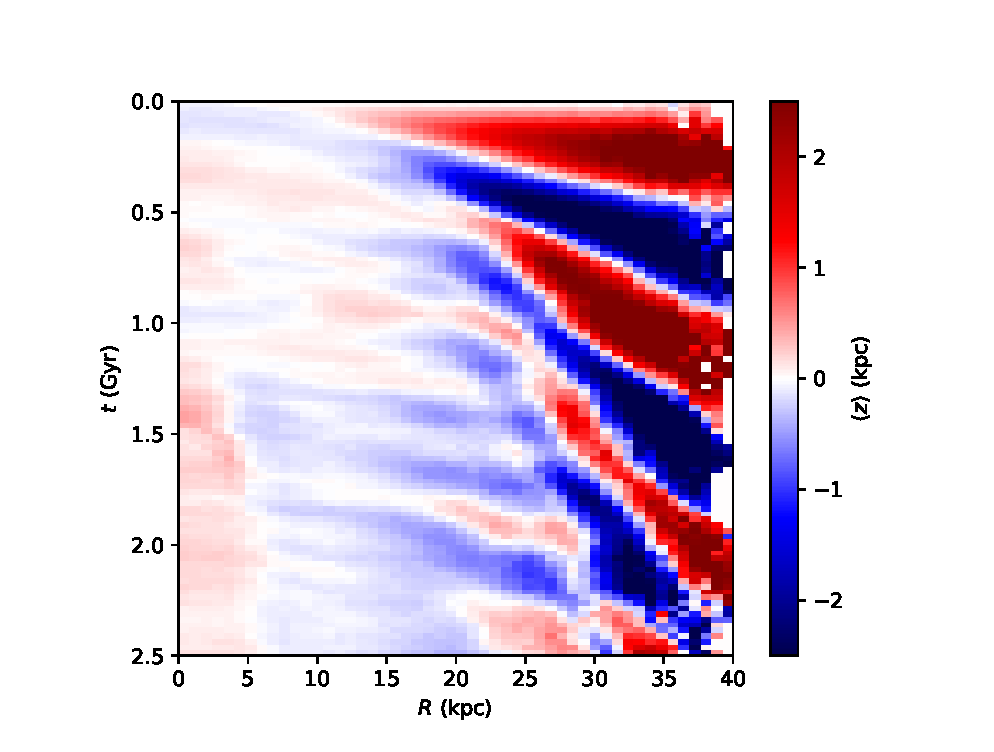
\includegraphics[width=0.8\textwidth]{../figures/isolated_z_0_r_a.eps}
	\caption{Mean height, $\langle z \rangle$ of the disc from the toy model described in \S\ref{ssec:toy_model_1} as a function of cylindrical radius and time.} \label{fig:toy_model_1_mean_height}
\end{figure}

\begin{figure}
	\centering
	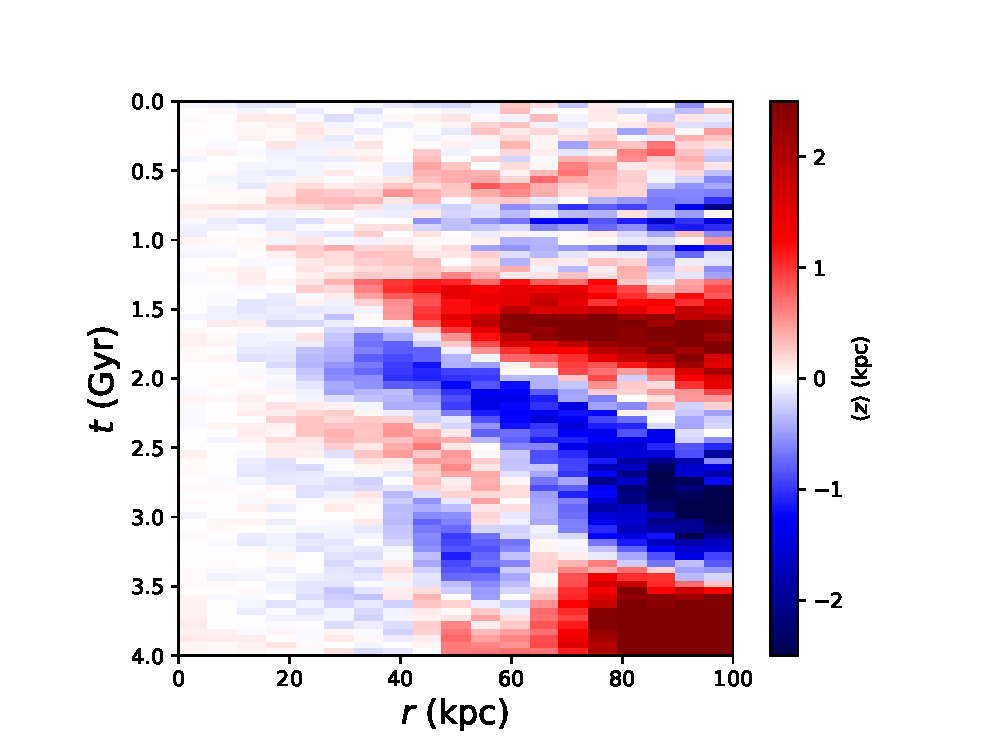
\includegraphics[width=0.8\textwidth]{../figures/isolated_z_0_r_a_halo.eps}
	\caption{Mean height, $\langle z \rangle$ of the halo from the toy model described in \S\ref{ssec:toy_model_1} as a function of spherical radius and time.} \label{fig:toy_model_1_mean_height_halo}
\end{figure}


\section{Overview} \label{sec:overview}


In this section, we illustrate the factors driving vertical structure in stellar discs with two toy models.
\subsection{Quantifying Structure in Discs}
%\vspace{0.6in}

The analysis of simulated galaxies invariably involves computing averages of physical quantities, namely functions of the phase-space coordinates, $\textbf{r}$ and $\textbf{v}$. For some observable function,  $\Theta(\textbf{r},\textbf{v})$, the average in a region $S$ is,
\begin{eqnarray}
\langle\Theta\rangle_S &=&\frac{1}{M_S} \int_S \text{d}^3 \textbf{r} \text{d}^3\textbf{v} f(\textbf{r}, \textbf{v}) \Theta(\textbf{r}, \textbf{v})\\
&\approx& \frac{1}{M_S} \sum_{j \in S} m_j \Theta(\textbf{r}_j, \textbf{v}_j) \label{eq:z_statistic}
\end{eqnarray}
where $M_S$ is the mass in $S$, $f(\textbf{r},\textbf{v})$ is the phase space distribution function, and $m_j$ is the mass of the $j$-th particle in $S$. For stellar discs, we are often interested in the Fourier series representation of $\Theta$ to quantify $m$-fold angular symmetries in some annulus with mean radius, $R_S,$
\begin{equation}
\langle\Theta(R_S,m)\rangle_S = \frac{1}{M_S} \sum_{j \in S} e^{i m \phi_j} m_j \Theta(\textbf{r}, \textbf{v})
\end{equation}
where $m$ is the degree of symmetry, and $\phi_j$ is the azimuthal angle of particle $j$. When $\Theta = z^n$, we call the average $Z_m^n$. We make extensive use of this form for this paper.

\subsection{Toy Model: Acceleration Along the Symmetry Axis} \label{ssec:toy_model_1}


For our first simulation, we study the vertical structure that is excited when a dark matter subhalo falls along the disc symmetry axis from a height of 100 kpc.  We generate the initial conditions using  the \textsc{GalactICS} code \citep{KGGalactICSReference,WPDGalactICSReference}, and simulate the system using \textsc{Gadget-3}, a privately released version of the popular \textsc{Gadget-2} code \citep{GadgetCodePaper}.

% This experiment is similar to Sellwood 1996...
The disc has an exponential surface density with scale length $R_d=3.7\,\kpc$ and mass $M_d=4\times10^{10} \,\solarm$. The halo is taken to be NFW, with scale length $R_h=33.2\,\kpc$, virial mass $M_h=1.1\times10^{12}$, and concentration $c=6.7$\footnote{The parameters for the halo are taken to be a sphericalized version of simulation B.Late in Table \ref{tab:sims}. This simulation will be described in more detail in \S\ref{sec:description}.}. We use $10^6$ halo particles and $3.5 \times 10^{6}$ disc particles. The subhalo is also assumed to be NFW with scale length $R_h=1.70\,\kpc$, virial mass $M_h=2.7\times10^{10}$, and concentration $c=38.1$\footnote{ The parameters for the substructure are given by B.Late.a in Table \ref{tab:substructure}.}. The subhalo is given a height of $z=100\,\kpc$ and zero velocity.



A disc-centered mean height map for disc particles is shown in Fig. \ref{fig:toy_model_1_mean_height}. Initially the disc remains relatively unperturbed; the subhalo is far enough away to exert a somewhat uniform acceleration across the disc. Only in the very outer disc do we see very slight disc flapping. As the subhalo makes its first pericentre, the inner disc is dragged toward the subhalo more strongly, causing a strong lag in the outer disc. After the subhalo has passed through the disc, the pattern reverses as the center of the disc is pulled back down. The resultant lag of the outer disc then shows up as a positive signal.



The oscillation pattern seen in Fig. \ref{fig:toy_model_1_mean_height} is not stationary in time, but rather becomes more complicated as time goes on. Immediately after the displacement first changes signs, the pattern starts to propagate outwards more slowly as evidenced by decreasing (increasing magnitude) slope of the ridges. The mean height shows oscillating single fixed-point standing wave behaviour, at some points (around 1 Gyr) appearing to gain another node.  As the system equilibrates, the $m=0$ disturbances are pushed further to the outer disc, but the magnitude of the perturbations remains high.

Qualitatively similar behaviour can be seen in the halo. Fig. \ref{fig:toy_model_1_mean_height_halo} shows the mean height of spherical shells in the halo. It paints a similar picture to the disc; the inner shells are dragged with the disc as the substructure pulls on the inner disc-halo system more strongly, while the outer halo lags the oscillations. The shells in the outer halo are displaced with longer periods of oscillation than in annuli in the outer disc, indicating a more complicated interaction with the substructure and inner disc-halo system. The halo develops multiple nodes in mean height by the end of the simulation, suggesting a similar standing wave-like phenomenon is occurring in the halo.

What is interesting about this experiment is the very long-lived nature of the flapping in the disc. Vertical instabilities are generally expected to phase mix, causing the disc to thicken. The flapping in our disc persists for longer than a dynamical time. In fact, a similar observation was made in an experiment performed by \citet{sellwood_1996} where a disc with similar properties was given an initial bulk displacement that varied as a function of radius. While other bending behaviour is rapidly suppressed, a flapping motion remained in the perturbed disc. Qualitatively, the results of \citet{sellwood_1996} are similar in magnitude to our own, suggesting that flapping naturally arises from near-axisymmetric perturbations of the disc.

\begin{figure}
	\centering
	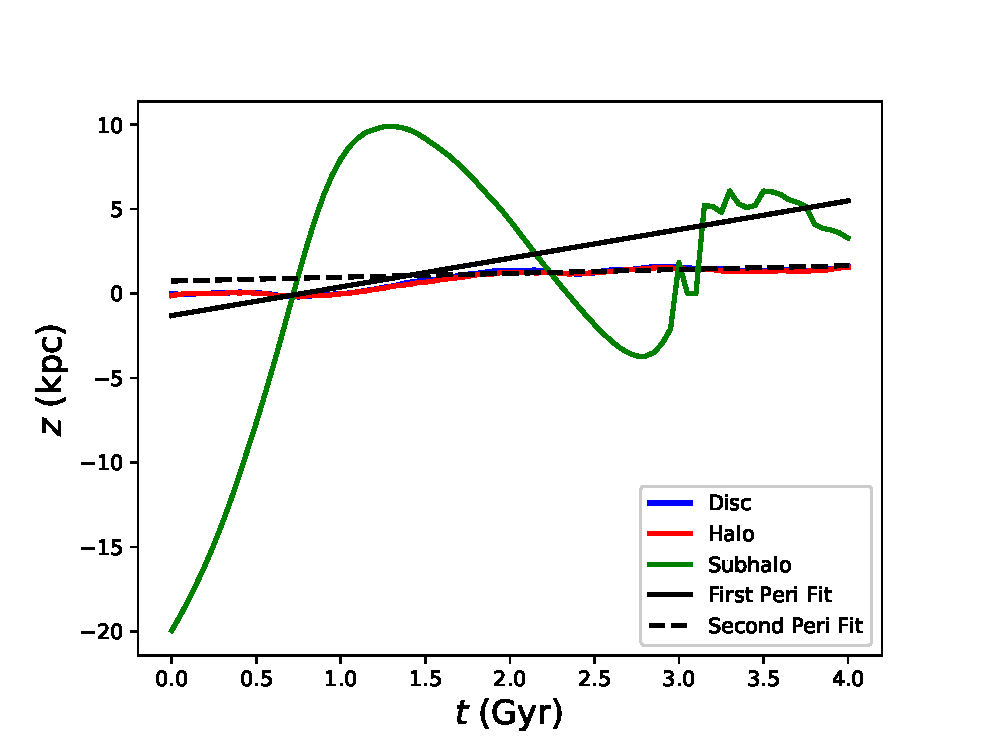
\includegraphics[width=0.8\textwidth]{../figures/isolated_orbits_two_fits.eps}
	\caption{The orbit of the disc (blue), halo (red), and subhalo(green) peak densities of the toy model described in \S\ref{ssec:toy_model_2}. The dashed black lines show the fits described in the text.} \label{fig:toy_model_2_orbits}
\end{figure}



\subsection{Toy Model: Massive Subhalo Interaction} \label{ssec:toy_model_2}
\begin{figure}
	\centering
	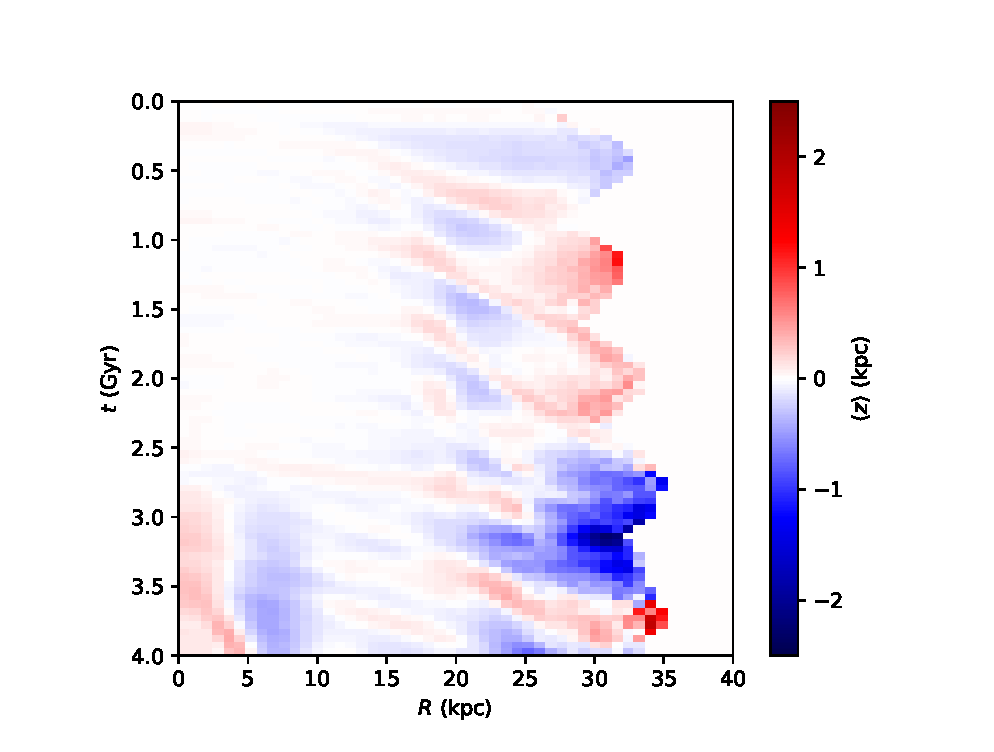
\includegraphics[width=0.8\textwidth]{../figures/b_late_light_subhalo_z_0_r_a.eps}
	\caption{Mean height, $\langle z \rangle$ of the disc from the toy model described in \S\ref{ssec:toy_model_2} as a function of radius and time.} \label{fig:toy_model_2_mean_height}
\end{figure}


Here, we present a more complicated satellite encounter. The orbit is inspired by a satellite in one of our cosmological simulations, and shows a massive satellite on a close orbit with the disc, passing through the midplane several times. The parameters for the disc, halo, and subhalo are the same as in \S\ref{ssec:toy_model_1}.


We plot the $z$ coordinate of the subhalo, disc, and halo peak densities in Fig. \ref{fig:toy_model_2_orbits}.
Initially, the subhalo is far from the disc at over 100 kpc, and about 20 kpc above the disc in $z$. We see the disc and halo peak densities track each other almost exactly over the course of the simulation, consistent with Fig. \ref{fig:toy_model_1_mean_height} and Fig. \ref{fig:toy_model_1_mean_height_halo}. In some short frame of time, we suggest that this system can be viewed as a two body problem between the disc-halo system and subhalo. That is, we have motion described by,
\begin{equation}
\frac{M_{dh}\textbf{r}_{dh} +  + M_{sh} \textbf{r}_{sh}}{M_{dh} + M_{sh}} = \textbf{r}_{c,0} + \textbf{v}_{c,0} t
\end{equation}
where $M_{dh}$ is the implied two-body disc-halo mass, $M_{sh}$ is the implied two-body subhalo mass, $\textbf{r}_{dh} = (M_d \textbf{r}_d + M_h \textbf{r}_h)/M_{dh}$, $\textbf{r}_d$ is the disc peak density position, $\textbf{r}_h$ is the halo peak density position, $\textbf{r}_{sh}$ is the subhalo peak density position, $\textbf{r}_{c,0}$ is the initial implied center of mass, and $\textbf{v}_{c,0}$ is the implied center of mass velocity.

We can find the density modes from the particle distributions each time very easily. However, $M_{dh}$, $M_{sh}$, $\textbf{r}_{c,0}$, and $\textbf{v}_{c,0}$ are unknowns. We maximize the likelihood,
\begin{equation}
\ln \mathcal{L} = \left\vert \frac{M_{dh}\textbf{r}_{dh} +  + M_{sh} \textbf{r}_{sh}}{M_{dh} + M_{sh}} - \textbf{r}_{c,0} + \textbf{v}_{c,0} t \right\vert^2 \, \text{kpc}^{-2}
\end{equation}
in two 1.0 Gyr windows  centered on 0.5 Gyr and 2.0 Gyr, respectively. These windows are chosen since they encompass the time before pericentric passages at 0.85 Gyr and 3.0 Gyr, when the subhalo is losing the most mass. The idea is that during pericentric passages, we expect the system to be poorly described by a two-body fit. The two center of mass motion lines, $\textbf{r}_{c,0} + \textbf{v}_{c,0} t$ are shown as the solid black and dashed black lines in Fig. \ref{fig:toy_model_2_orbits}, respectively. We imply effective two-body mass ratios of 16.3:1 and 85.0:1, respectively, for disc-halo:subhalo masses. 

The likelihood represents the mean distance deviation from our fit. For the two windows centered at 0.5 Gyr and 2.0 Gyr, we have the average root-log-likelihood $(N^{-1}\ln\mathcal{L})^{1/2}= 0.19$ in the first window and  $(N^{-1}\ln\mathcal{L})^{0.5} = 0.29$ in the second, where $N$ is the number of observations in the window. We thus infer small deviations from a two body problem when the subhalos are not at pericenter, implying that this model describes the data well.  We submit this technique as a way to quantify the effect of inertial acceleration in isolated satellite encounters. Although the drift velocity of the system changes as the satellite sheds mass, the picture is clear: the disc is placed on an oscillating orbit in $z$, and is no doubt subject to differential vertical acceleration. Despite this acceleration, the disc axis as measured by its moment of inertia tensor is relatively undeflected, being constrained to less than $2^{\circ}$ in the first 4 Gyr.


We see the orbit's effect on the mean height of the disc in Fig. \ref{fig:toy_model_2_mean_height}. At the beginning of the simulation, although the amplitude of the oscillations is lower, we see qualitatively similar behaviour to the first toy model. There is no obvious mean height bump when the substructure is at pericenter, indicating that passages through the disc plane are less substantial for generating $m=0$ corrugations than the overall two-body orbit. We expect that any subhalo capable of creating two-body motion of the disc along the disc axis will generate substantial, several hundred parsec corrugations. 


\section{Description of Experiments} \label{sec:description}



In this section, we proceed to generalize to a fully cosmological environment. 

\begin{figure}
	\centering
	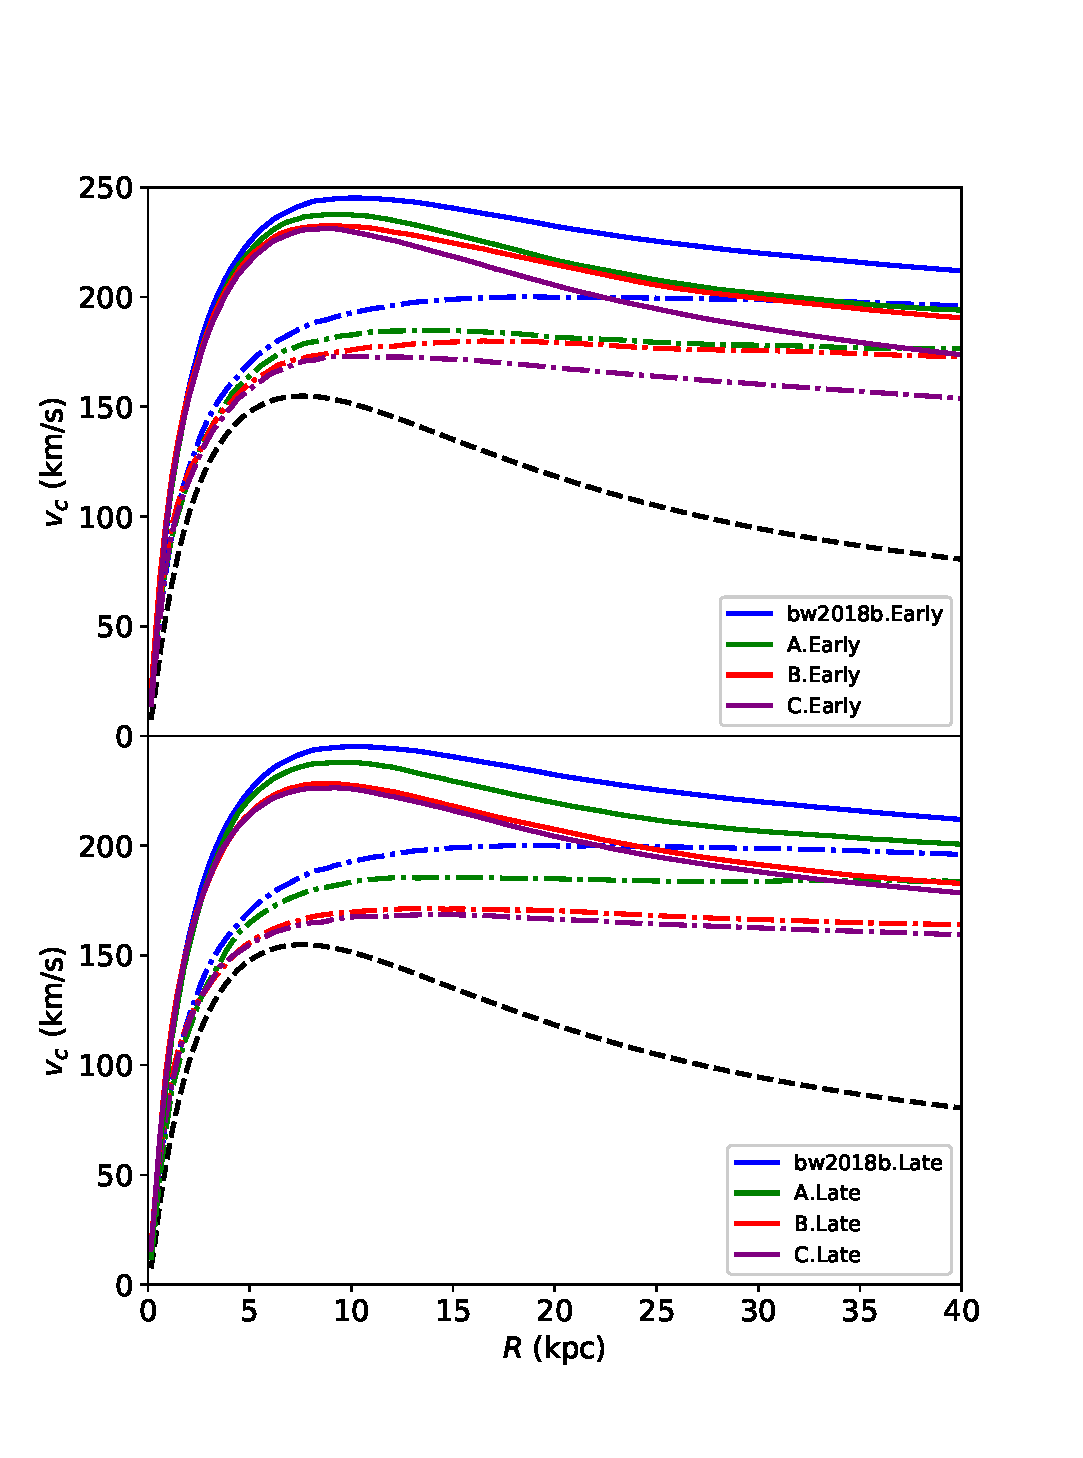
\includegraphics[width=0.8\textwidth]{../figures/rotation_curve.eps}
	\caption{The rotation curves for all considered models. The same disc is used in all runs, and its rotation curve contribution shown by the black dashed line. The halo contributions  for the Early and Warm subsuites are shown in the top panel as dot-dashed lines, with the total rotation curves being solid. The bottom panel shows the same for the Late subsuite.} \label{fig:rotation_curves}
\end{figure}



\begin{figure}
	\centering
	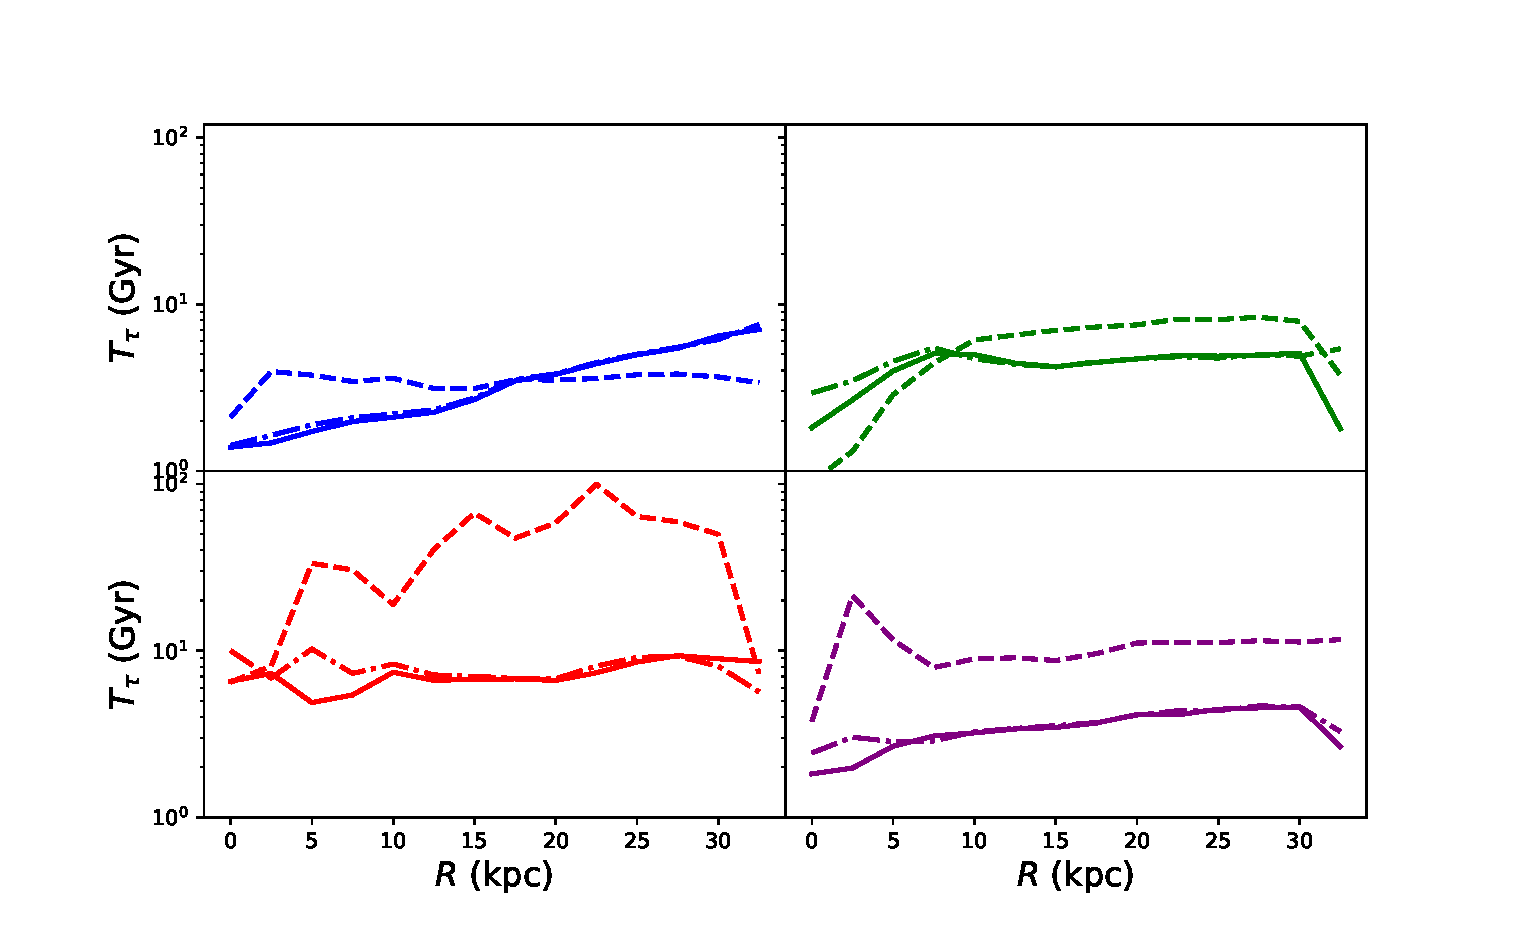
\includegraphics[width=0.8\textwidth]{../figures/timescale.eps}\caption{The timescale of torque acting on a ring for all models considered in this paper. Colours are the same as in Fig. 5. Line types are Early (solid), Warm (dot-dashed), and Late (dashed).} \label{fig:ratio_freqs}
\end{figure}

\begin{figure}
	\centering
	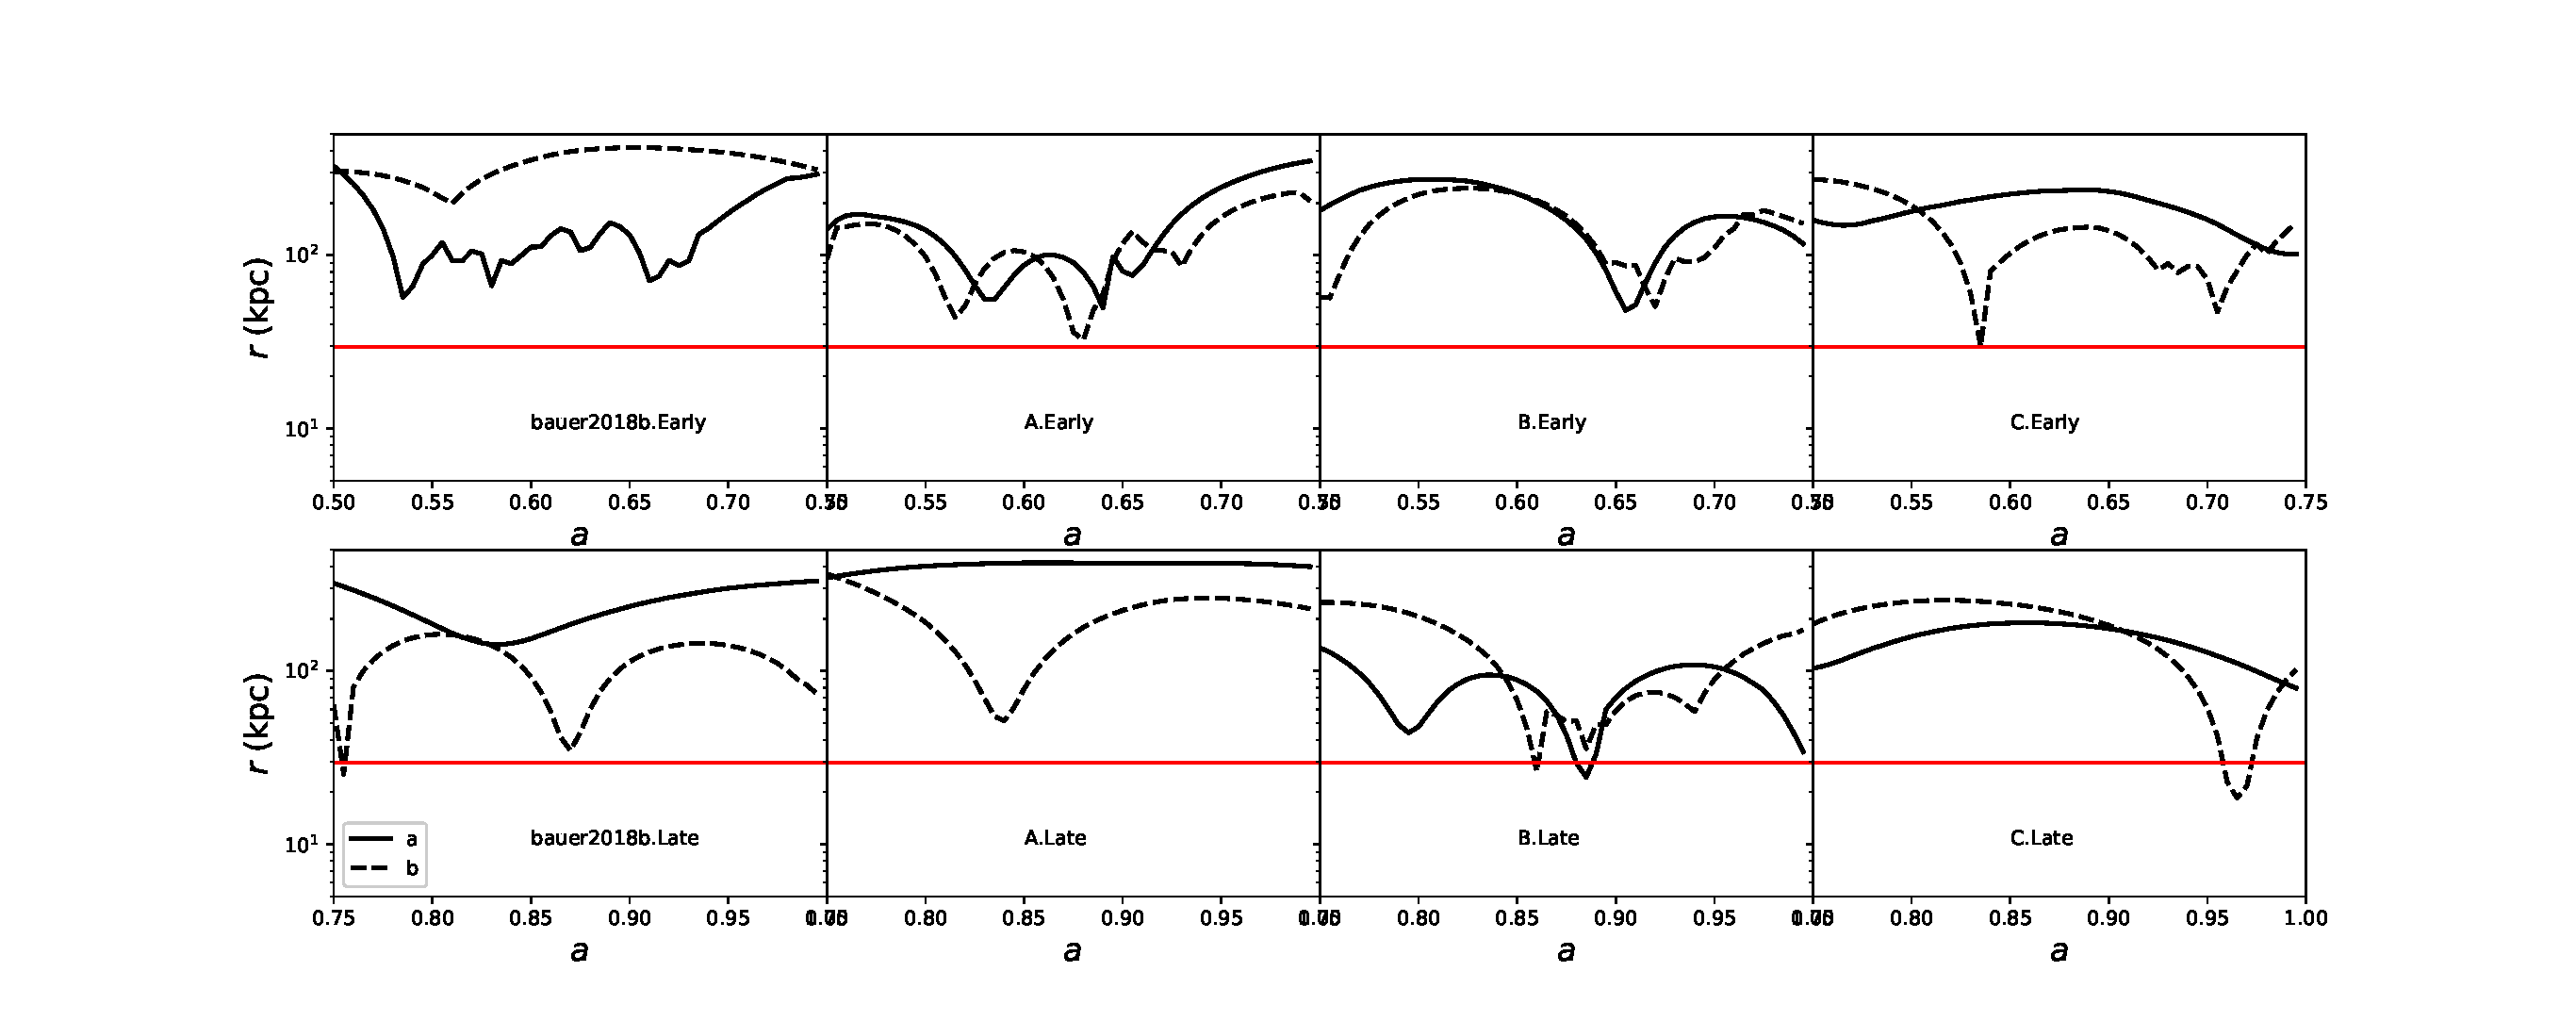
\includegraphics[width=0.8\textwidth]{../figures/substructure_r_vs_t.eps}
	\caption{The orbits of the two most massive structures at initialization for the fiducial suite (top panel) and the late insertion suite (bottom). These are the substructures listed as the top two entries for each simulation in Table \ref{tab:substructure}. The red line denotes $20\, \kpch = 29.5 \, \kpc$. } \label{fig:substructure_orbits}
\end{figure}

\subsection{Disc Insertion Technique} \label{ssec:disc_insertio}

Our disc insertion scheme is described in \citet{bauer2018a}, and
it expands upon method introduced by
\citet{BerentzenShlosmanStellarDisks}, \citet{debuhr_2012}, and
\citet{ys_2015}. Our scheme uses an iterative procedure to
initialize an axisymmetric, smooth disc in a cosmological halo, generally clumpy and triaxial. 
The first step is to run a pure dark matter
simulation and identify a suitable halo.  We then rerun the simulation with a rigid disc potential which 
grows from an initial scale factor, $a_g$, to a final scale factor, $a_l$.
When the simulation reaches $a_l$,
the rigid disc is replaced by an N-body system and the ``live'' disc-halo
system is evolved to the present epoch. 

For our pure dark matter simulation, we implement the zoom-in
technique of \citet{KatzQuasarZoom} and \citet{NavarroWhiteZoom}.
Selecting for Milky Way-like halos with no major mergers, we use the
results of \cite{onorbe_etal_2014} to ensure no low-resolution particle contamination.
We choose cosmological parameters based on the results
from Planck 2013 \citep{planck_2014} with $H_0=67.9\,{\rm
  km\,s}^{-1}\,{\rm kpc}^{-1}$, $\Omega_b = 0.0481$, $\Omega_0 =
0.306$, $\Omega_\Lambda = 0.694$, $\sigma_8 = 0.827$, and $n_s =
0.962$.  N-body initial conditions for the dark matter particles are
generated with the \textsc{music} code \citep{music}.  

%We select a suitably-sized halo for a Milky Way-like galaxy, namely
%one with a $z=0$ mass of $1.23\times 10^6\,h^{-1} M_\odot$
%that comprises $10^6$.

During its growth phase from $a_g=0.25$ to $a_l=0.5$\footnote{For reference, $a=0.5$ is 5.9 Gyr after the Big Bang, and $a=0.75$ is 10.0 Gyr after the Big Bang. The age of this Universe at present day is 13.8 Gyr.}, the disc is treated
as a rigid body whose orientation and center-of-mass position evolve
according to the standard equations of rigid body dynamics. \citet{bauer2018a} found that
the rigid disc assumption is actually quite true to the orientation
and center of mass evolution of a pure stellar disc. At
$a_l$, we swap a live disc for the rigid one using a modified version of
\textsc{GalactICS} \citep{KGGalactICSReference,WPDGalactICSReference}, which generates a
three-integral DF disc in the best axisymmetric approximation to the
halo \citet{bauer2018a}.


\subsection{Numerical Experiments} \label{ssec:numerical_experiments}

%We apply the technique described in \S \ref{ssec:disc_insertio} to understand a possible disc origin of low-latitude streams, and more generally how vertical structure evolves in pure stellar discs. In particular, we are interested in understanding how, in a cosmological simulation, stars are kicked up out of the disc. They comprise a component, if not all member stars of low-latitude streams. We discuss useful definitions of this population subsequently in \S\ref{ssec:def}. Such kicked-up disc stars (KUD stars) may be useful probes of the Galactic potential if we can understand how their orbits were altered.

We present a concise description of our cosmological models in Table \ref{tab:sims}. The haloes are chosen such that the total circular speed curves are similar to the Milky Way's. One of the haloes is considered by \cite{bauer2018b}, and the other three, A, B, and C, are previously unpublished.
 
Fig. \ref{fig:rotation_curves} shows the circular speed curves for all disc-halo combinations. The top panel shows these for our fiducial suite of simulations, which has $a_l=0.5$. This suite of simulations is denoted for halo X as X.Early. We also run a suite of simulations with $a_l=0.75$, and the corresponding circular speed curves are shown in the bottom panel. This suite is denoted as X.Late. We see a submaximal disc in all cases, and a relatively small spread in circular velocities in the inner disc. In particular, the ratio of the square of the disc contribution to the rotation curve and square of the total rotation curve measured at $2.2\, R_d$, $\left. V_d^2/V_{tot}^2 \right \vert_{R=2.2\,R_d}$, ranges between 0.37 and 0.46. These values are far below the lower bound for a maximal disc as advocated by \citet{sackett_1997}. 

One of the benefits of disc insertion techniques is the ability to modify disc properties in the same halo. We exploit this in our third suite denoted as X.Warm. In this suite, we have increased the disc's dynamical temperature measured by Toomre $Q$ \citep{toomre_q}.

Although we explore all of our models in \S\ref{sec:evolution} and \S\ref{sec:kud}, we identify three key simulations for further study in \S\ref{sec:disentangle}.
\begin{enumerate}
\item \textbf{Strong Subhalo Interaction:} B.Late has a close interaction with two subhaloes, but no substantial disc-halo misalignment. One of these subhaloes passes twice through the plane of the disc, one time interior to 30 kpc.
\item \textbf{Disc-Halo Misalignment:} C.Early presents a case with no massive subhalo interactions, but a substantial misalignment from its host halo.
\item \textbf{Distant Massive Subhaloes:} A.Early is relatively aligned to its host halo, but its most massive substructures do not interact closely with the disc.
\end{enumerate}
These simulations represent three archetypal halo environments, which we explore in more detail in subsequent sections.



\begin{sidewaystable}
\centering
\caption{Table of simulations run in the main experiment. $M_h$ is the virial mass of the host halo, $R_h$ is the NFW scale length of the host halo, $c$ is the NFW concentration parameter of the host halo, $a_l$ is the live disc insertion scale factor, $\delta \Theta_{h,20}$ is the halo misalignment angle for the 20 kpc shell, $N_d$ is the number of disc particles,  $Q$ is the Toomre stability parameter of the disc at initialization, and $f_{kud}$ is the fraction of disc mass that gets classified as KUD stars measured at present day with $\eta=8$.} \label{tab:sims}
\begin{tabular}{l l l l l l l l l l}
\hline
       & $M_h\,\,(\solarm)$ & $R_h\,\,(\kpc)$ & $c$ & $a_l$ &  $N_d$ & $Q$ & $\cos\delta \Theta_{h,20}$ & $f_{kud}$\\
\hline
bauer2018.Early   & $1.0 \times 10^{12}$ & 15.9 &  9.84 &   0.50 & $1.0 \times 10^6$ & 1.1 & 0.16 & $1.2 \times 10^{-2}$\\
bauer2018.Warm    & $1.0 \times 10^{12}$ & 15.9 &  9.84 &   0.50 & $1.0 \times 10^6$ & 1.1 & 0.16 & $1.1 \times 10^{-2}$\\
bauer2018.Late    & $1.2 \times 10^{12}$ & 15.2 &  15.4 &   0.75 & $1.0 \times 10^6$ & 1.8 & 0.93 &$4.2 \times 10^{-3}$\\
A.Early           & $9.4 \times 10^{11}$ & 17.8 &  8.56 &   0.50 & $3.5 \times 10^6$ & 1.3 & 0.97 &$3.7 \times 10^{-3}$\\
A.Warm            & $9.4 \times 10^{11}$ & 17.8 &  8.56 &   0.50 & $3.5 \times 10^6$ & 1.8 & 0.97 & $1.6 \times 10^{-3}$\\
A.Late            & $1.1 \times 10^{12}$ & 18.5 &  12.1 &   0.75 & $3.5 \times 10^6$ & 1.3 & 0.98 & $6.8 \times 10^{-5}$\\
B.Early           & $5.9 \times 10^{11}$ & 10.4 &  12.6 &   0.50 & $3.5 \times 10^6$ & 1.3 & 0.91 & $8.5 \times 10^{-4}$\\
B.Warm            & $5.9 \times 10^{11}$ & 10.4 &  12.6 &   0.50 & $3.5 \times 10^6$ & 1.8 & 0.91 & $1.2 \times 10^{-3}$\\
B.Late            & $1.1 \times 10^{12}$ & 33.2 &  6.70 &   0.75 & $3.5 \times 10^6$ & 1.3 & 0.99 & $9.2 \times 10^{-4}$\\
C.Early           & $4.3 \times 10^{11}$ & 8.33 &  14.1 &   0.50 & $3.5 \times 10^6$ & 1.3 & 0.84 & $5.3 \times 10^{-3}$\\
C.Warm            & $4.3 \times 10^{11}$ & 8.33 &  14.1 &   0.50 & $3.5 \times 10^6$ & 1.8 & 0.84 & $5.6 \times 10^{-3}$\\
C.Late            & $6.7 \times 10^{11}$ & 13.6 &  14.0 &   0.75 & $3.5 \times 10^6$ & 1.3 & 0.92 & $1.0 \times 10^{-4}$\\
\hline
\end{tabular} 

\end{sidewaystable}

\subsection{Halo Environments} \label{ssec:halo_env}


%As mentioned in \S\ref{ssec:numerical_experiments}, the haloes we consider are meant to resemble the Milky Way. In Table \ref{tab:sims}, all of the simulations we consider are listed. 


%In addition to basic properties like halo mass, $M_h$, and scale radius, $R_h$, we also want to know how equilibrated the halo is with the disc. Discs will tumble in response to an external specific torque, $\boldsymbol \tau$, induced by the non-equilibrated halo. This invariably produces vertical structure.

Here, we further quantify our halo environments in terms of the effects we expect their smooth distributions and subhalos to have on the disc. For the former of these, we examine the following timescale,
\begin{equation}
T_\tau = \frac{L(R)}{\tau_\perp(R)},
\end{equation}
where $L(R)$ is the magnitude of the angular momentum in a ring centered at radius $R$, and $\tau_\perp(R)$ is the cylindrically averaged perpendicular torque in an annulus centered at $R$. This timescale is plotted as a function of radius at initialization for our models in Fig. \ref{fig:ratio_freqs}. This lower the timescale, the more the initial halo configuration contributes to the relevant torque. For example, we would interpret the simulation C.Early as being substantially non-equilibrated at initialization. Generally speaking, the more misaligned disc-halo systems have shorter torque action timescales. The effect of having a warmer disc is most pronounced in the inner regions, where the increased angular momentum from asymmetric drift appears to increase $T_\tau$.

%In a non-equilibrium state, shells of the halo may be misaligned from others at different radii. This creates a torquing effect on the disc and causes it to reorient (see \cite{DubinskiKuijkenRigidDisks}, for example). Torques present an opportunity for the angular momenta of orbits to change, and may result in the generation of KUD stars. Fig. \ref{fig:disk_torques} shows the specific torque as a function of radius for all models. In the most misaligned simulations, bauer2018b.Early/Warm, bauer2018b.Late, and C.Early/Warm, there is an obvious torque signature in the intermediate parts of the disc.

%he relative tilt of the halo principal axes compared to the halo interior for all runs. The model considered in \citet{bauer2018b}, bauer2018b.Early stands out the most. It shows substantial misalignment at all radii. C.Early also shows substantial misalignment, but the other simulations seem to have mostly aligned short axes.\
 
Subhalo interactions pose another potential source of perpendicular torque. We expect the timescales over which these events act to be shorter, but we can understand them by looking at the subhalo orbits directly. Fig. \ref{fig:substructure_orbits} shows the two most massive substructures in a plot of $r$ vs $t$ for all runs. A list of the top five most massive (at initialization) substructures' masses and scale radii is presented in Table \ref{tab:substructure}. The orbits present a wide variety of behaviour. For example, the subhaloes in bauer2018b.Early live most of their lives in the outer halo on roughly tangential orbits. Opposite to this are radial orbits like the one of C.Late.b, for example. Of course, most orbits exist somewhere in between on this scale. 


\begin{sidewaystable}
\caption{Table of the five most massive substructures at $a_l$ in all of the simulations detailed in Table \ref{tab:sims}. The virial mass, $M_s$, and NFW scale radius, $R_s$, are given.}\label{tab:substructure}
	\begin{tabular}{|l l l l | l l l l|}
	\hline
	Subhalo Name ($z=1$) & $M_s \,(\solarm)$ & $R_s \, (\kpc)$ & $c$ & Subhalo Name ($z=0.333$) & $M_s \,(\solarm)$ & $R_s \, (\kpc)$ & $c$\\	
	\hline
    bauer2018b.Early.a & $1.4 \times 10^{10}$ & 3.75 & 9.92 & bauer2018b.Late.a & $1.6 \times 10^{10}$ & 3.35 & 16.5 \\
    bauer2018b.Early.b & $1.0 \times 10^{10}$ & 1.02 & 32.8 & bauer2018b.Late.e & $0.7 \times 10^{10}$ & 0.27 & 154. \\
    bauer2018b.Early.c & $0.5 \times 10^{10}$ & 2.60 & 10.1 & bauer2018b.Late.c & $0.3 \times 10^{10}$ & 0.07 & 485. \\
    bauer2018b.Early.d & $0.4 \times 10^{10}$ & 1.51 & 15.7 & bauer2018b.Late.d & $0.3 \times 10^{10}$ & 1.06 & 29.8 \\
    bauer2018b.Early.e & $0.2 \times 10^{10}$ & 0.28 & 69.0 & bauer2018b.Late.e & $0.2 \times 10^{10}$ & 0.38 &  76.7\\
	\hline
	A.Early.a & $1.8 \times 10^{10}$ & 2.69 & 15.3 & A.Late.a & $1.3 \times 10^{10}$ & 2.62 & 19.6 \\
	A.Early.b & $1.2 \times 10^{10}$ & 1.26 & 28.4 & A.Late.b & $0.9 \times 10^{10}$ & 0.61 & 74.8 \\
	A.Early.c & $1.0 \times 10^{10}$ & 0.71 & 47.9 & A.Late.c & $0.5 \times 10^{10}$ & 0.77 & 46.4 \\
	A.Early.d & $0.7 \times 10^{10}$ & 2.29 & 13.0 & A.Late.d & $0.4 \times 10^{10}$ & 1.69 & 19.7 \\
	A.Early.e & $0.5 \times 10^{10}$ & 1.73 & 13.2 & A.Late.e & $0.2 \times 10^{10}$ & 1.25 & 21.5 \\
	\hline
	B.Early.a & $1.1 \times 10^{10}$ & 1.76 & 19.4 & B.Late.a & $2.7 \times 10^{10}$ & 1.70 & 38.1 \\
	B.Early.b & $0.2 \times 10^{10}$ & 0.41 & 47.5 & B.Late.b & $1.2 \times 10^{10}$ & 2.27 & 22.0 \\
	B.Early.c & $0.2 \times 10^{10}$ & 0.67 & 28.4 & B.Late.c & $0.6 \times 10^{10}$ & 2.67 & 14.4 \\
	B.Early.d & $0.2 \times 10^{10}$ & 1.81 & 10.3 & B.Late.d & $0.4 \times 10^{10}$ & 1.42 & 24.0 \\
	B.Early.e & $0.2 \times 10^{10}$ & 0.54 & 34.0 & B.Late.e & $0.4 \times 10^{10}$ & 1.13 & 29.7 \\
	\hline
    C.Early.a & $1.0 \times 10^{10}$ & 1.78 & 18.5 & C.Late.a & $0.5 \times 10^{10}$ & 0.18 & 194. \\
	C.Early.b & $0.6 \times 10^{10}$ & 0.92 & 30.0 & C.Late.b & $0.4 \times 10^{10}$ & 6.37 & 5.46 \\
	C.Early.c & $0.3 \times 10^{10}$ & 2.24 & 10.2 & C.Late.c & $0.4 \times 10^{10}$ & 0.75 & 46.2 \\
	C.Early.d & $0.1 \times 10^{10}$ & 0.91 & 18.7 & C.Late.d & $0.3 \times 10^{10}$ & 1.26 & 26.1 \\
	C.Early.e & $0.1 \times 10^{10}$ & 0.25 & 60.3 & C.Late.e & $0.3 \times 10^{10}$ & 6.78 & 4.81 \\
	\hline
	\end{tabular}
\end{sidewaystable}



\section{Structure and Evolution of Simulation Models} \label{sec:evolution}

We briefly summarize the evolution of the models in our simulation suite. We are especially interested in the time evolution of vertical density features in the discs.



\subsection{Bar Formation}


\begin{figure}
    \centering
	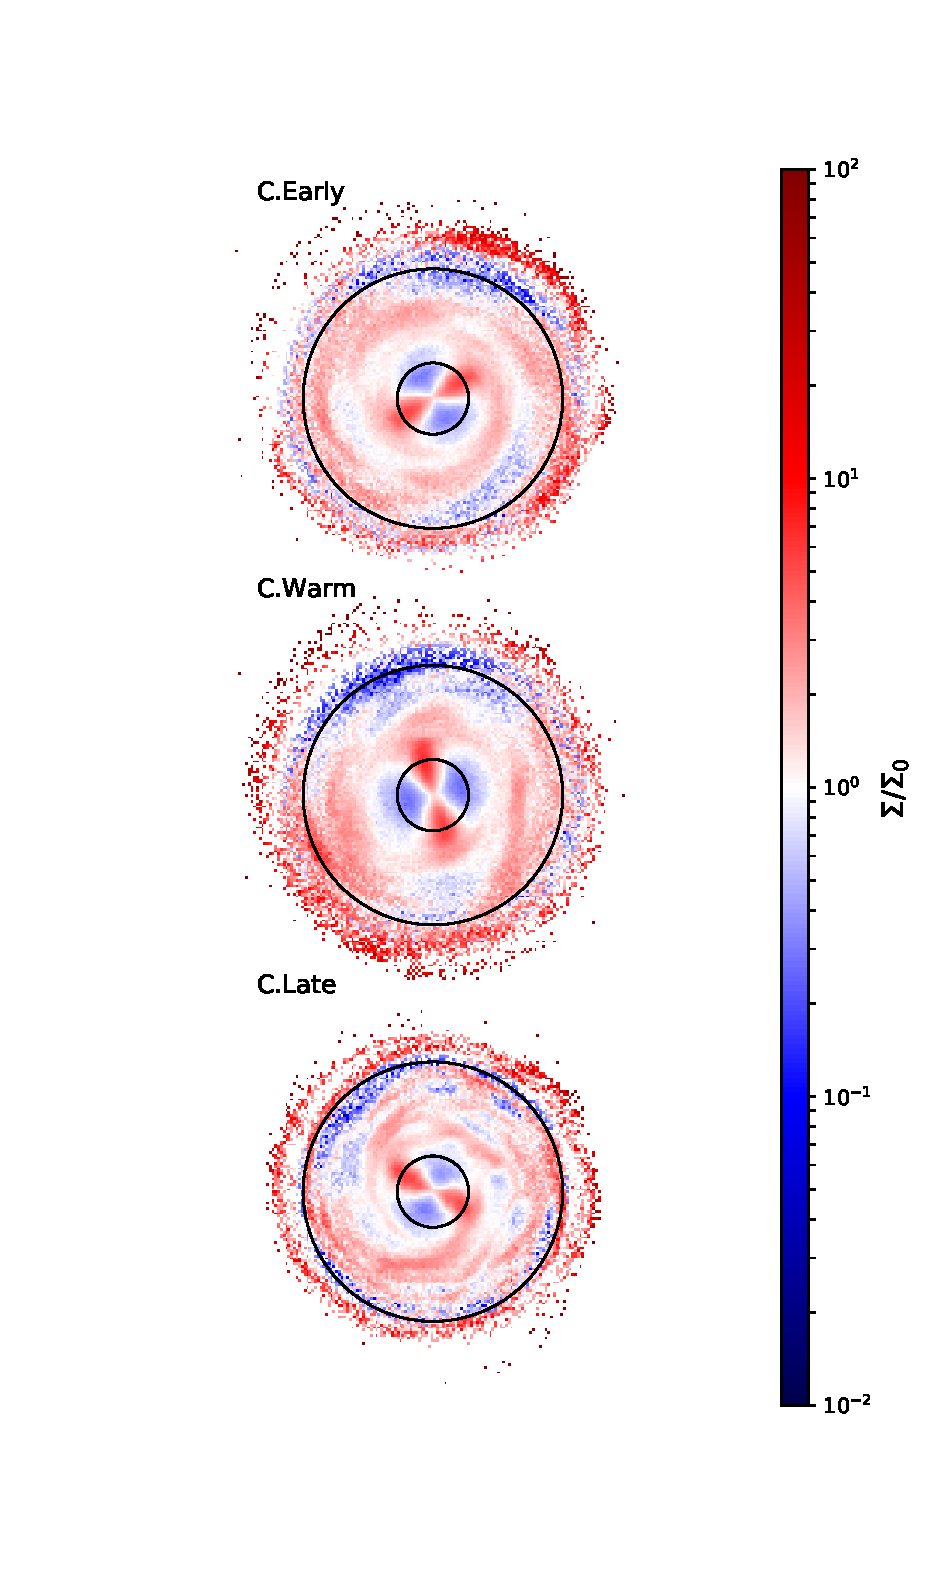
\includegraphics[width=0.8\textwidth]{../figures/surface_density_ratios.eps} \caption{The ratio of surface density, $\Sigma$, to azimuthally averaged surface density, $\Sigma_0$ for the C.Early, C.Warm, and C.Late models. The circles correspond to $R_p = 2.2\, R_d = 8.1 \,\kpc$ and $20 \,\kpch = 29.5 \, \kpc$.}
	\label{fig:final_densities}
\end{figure}

\begin{figure}
	\centering
	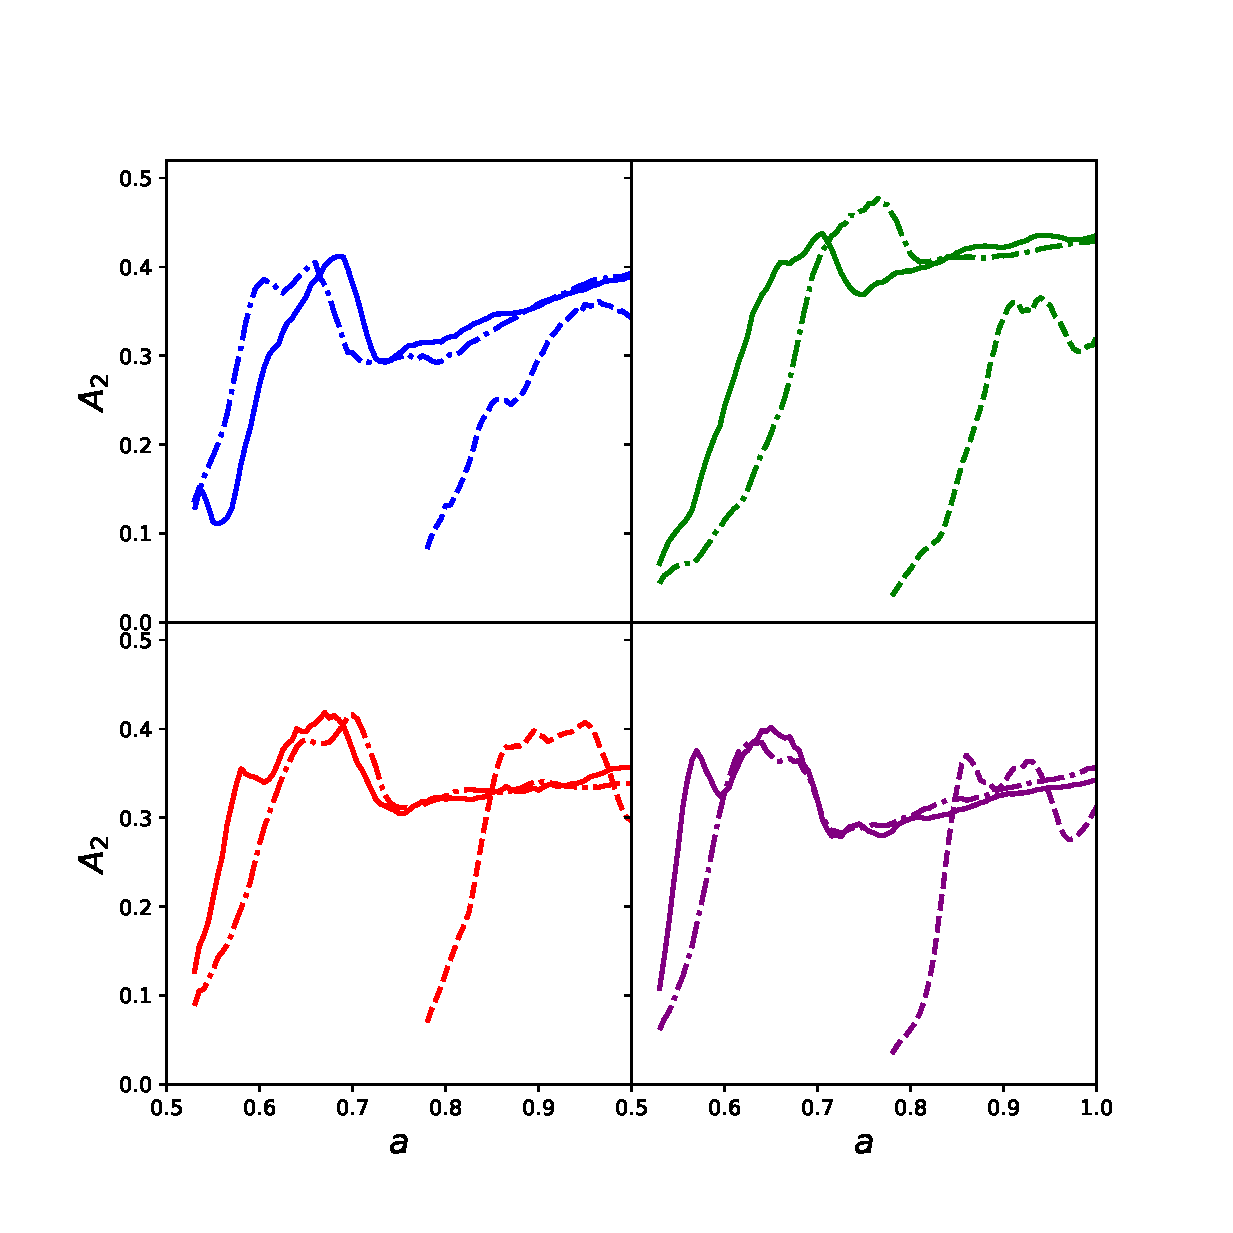
\includegraphics[width=0.8\textwidth]{../figures/a_2_all_models_four_panel.eps}
	\caption{Bar strength as measured by $A_2(<R_p)$ as a function of time for all models.} \label{fig:a_2}
\end{figure}



In isolation, a disc-halo system forms a bar when shot noise induced perturbations exponentially grow \citep{EfstathiouShotNoise}. Factors such as the relative contribution of the disc to the rotation curve, radial velocity dispersion, and disc scale height broadly determine bar formation rate, strength, and length \citep{AthanassoulaSellwood1986,ChristodoulouStability1995, Klypin2009, Sellwood2013, bauer2018b}. 
Strong environmental perturbers such as halo substructure and tides can induce bar formation even in discs that resist bar formation in isolation \citep{gauthier_2006, kazantzidis2008, purcell2011}. In similar studies using simpler disc insertion schemes, \citet{debuhr_2012,ys_2015} used a disc insertion scheme, and found that stellar discs always form bars in a cosmological environment, even if they are submaximal. \citet{ys_2015} found that the presence of a classical bulge substantially mitigated this conclusion. 


In a previous paper, we argued that these simulations overestimated the susceptibility of the disc to forming strong bars \citep{bauer2018b}. This argument stems from the initial thickness used in these studies, which we found to be a major factor in determining present-day bar strength. Specifically, this is because thin discs grow bars more quickly, and are able to buckle more easily, a process which regulates their strength. In contrast, thick discs grow their bars almost completely monotonically.


The final, present-day surface density excesses are shown in Fig. \ref{fig:final_densities}. Broadly speaking, our simulations form bars similar to the Milky Way's bar.  The bulk of the bar mass in all simulations appears contained to within $R_p = 2.2\, R_d$, as shown by visual inspection of the inner circles. Furthermore, it the warm suite is not substantially distinguishable upon inspection of this snapshot, indicating that the increased radial velocity dispersion did little to stop the formation of a bar in a cosmological setting.   The late-insertion suite shows a reduced bar length, bolstering an idea presented in \citet{bauer2018b} that for similar galaxies, one might be able to use the bar length to compare relative dates of stellar discs. Although we show only the the C.Early, C.Warm, and C.Late models, we find no substantial differences with other models within each subsuite.


In Fig. \ref{fig:a_2}, we plot the bar strength parameter (Eq. \eqref{eq:z_statistic} with $\theta=1$ and $m=2$)  evaluated in the region $R < R_p$ \citep{debattista_sellwood_2000}. First, we note that all models experience some kind of buckling event. We notice that the late suite appears to buckle lower magnitudes. Generally speaking, we see that the warm discs are delayed in their bar formation and buckling, although bauer2018b.Warm is an exception. The final bar strengths as measured by $A_2(R<R_p)$ are similar in magnitude, consistent with Fig. \ref{fig:final_densities}.



The picture painted between Fig. \ref{fig:final_densities} and Fig. \ref{fig:a_2} bolsters the previous claim that Milky Way discs in a cosmological environment will all form bars. Upon inspection, the bars are qualitatively similar to Milky Way's bar, suggesting no real problem on this front for a Milky Way thin stellar disc forming around or slightly after $z=1$. If the Milky Way took a similar trajectory to these simulations, it would not be unreasonable to suspect that observed vertical structure in the Milky Way is in part driven by a buckling bar.

\subsection{Disc Heating}
\begin{figure}
	\centering
	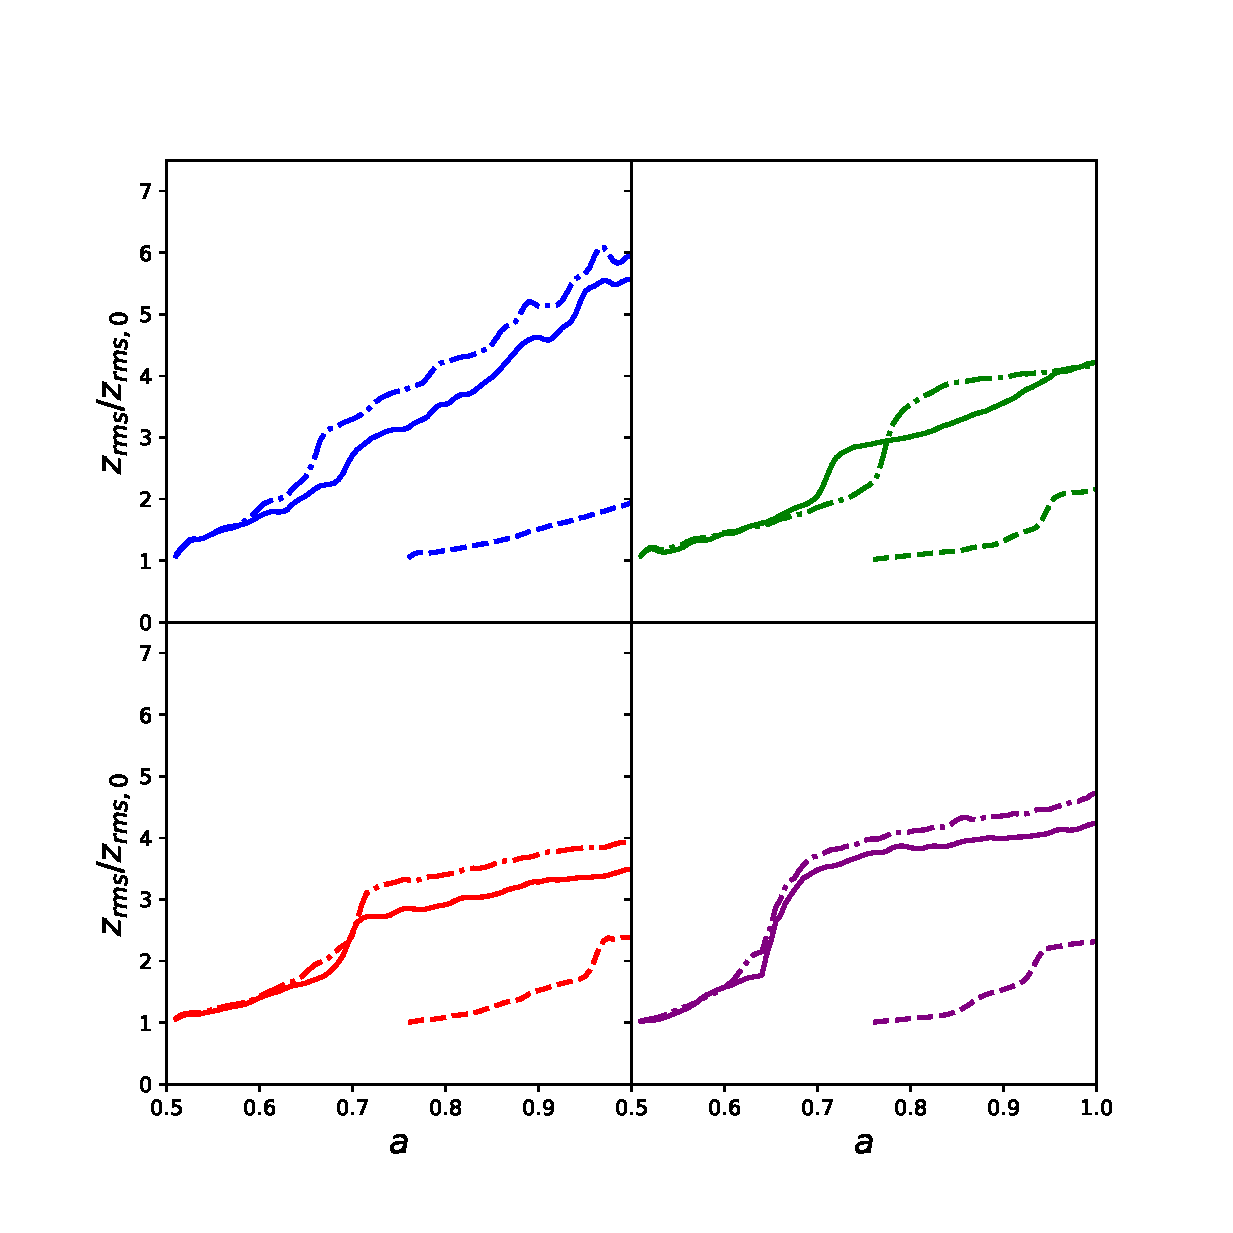
\includegraphics[width=0.8\textwidth]{../figures/z_rms_all_models_four_panel.eps}
	\caption{Disc height as measured by $z_{rms}/z_{rms,0}$ as a function of time for all models.} \label{fig:z_rms}
\end{figure}


The tendency for discs to thicken as they evolve, as measured by $z_{rms} = \sqrt{Z_2^0}$, is a well-studied phenomenon. In the secular evolution of galaxies, bars and spiral structure drive disc heating \citep{mcmillan_dehnen_2007,Sellwood2013}. Other sources of vertical heating include interactions with massive satellites and the cosmological environment \citep[for example]{lacey_ostriker_1985, toth_ostriker_1992, sellwood_1998, bauer2018b}. These two effects together suggest that we expect cosmological disc systems to thicken with time.
%\\

In fact, we see this confirmed in our simulations.  Fig. \ref{fig:z_rms} shows the evolution of $z_{rms}$ for each disc in the fiducial and warm suites. We see that substantial heating follows bar buckling in each simulation, a result consistent with \citet{ys_2015,bauer2018b}. We note that the warm suite exhibits up to 25\% more disc heating.  There is very little to say about the late-insertion scheme in this respect other than that the discs approximately double in height over the simulation time. These simulations end as the buckling process begins, and this may explain why vertical heating is more limited.\\

\subsection{Bending in Cosmological Discs}
\begin{figure}
    \centering
	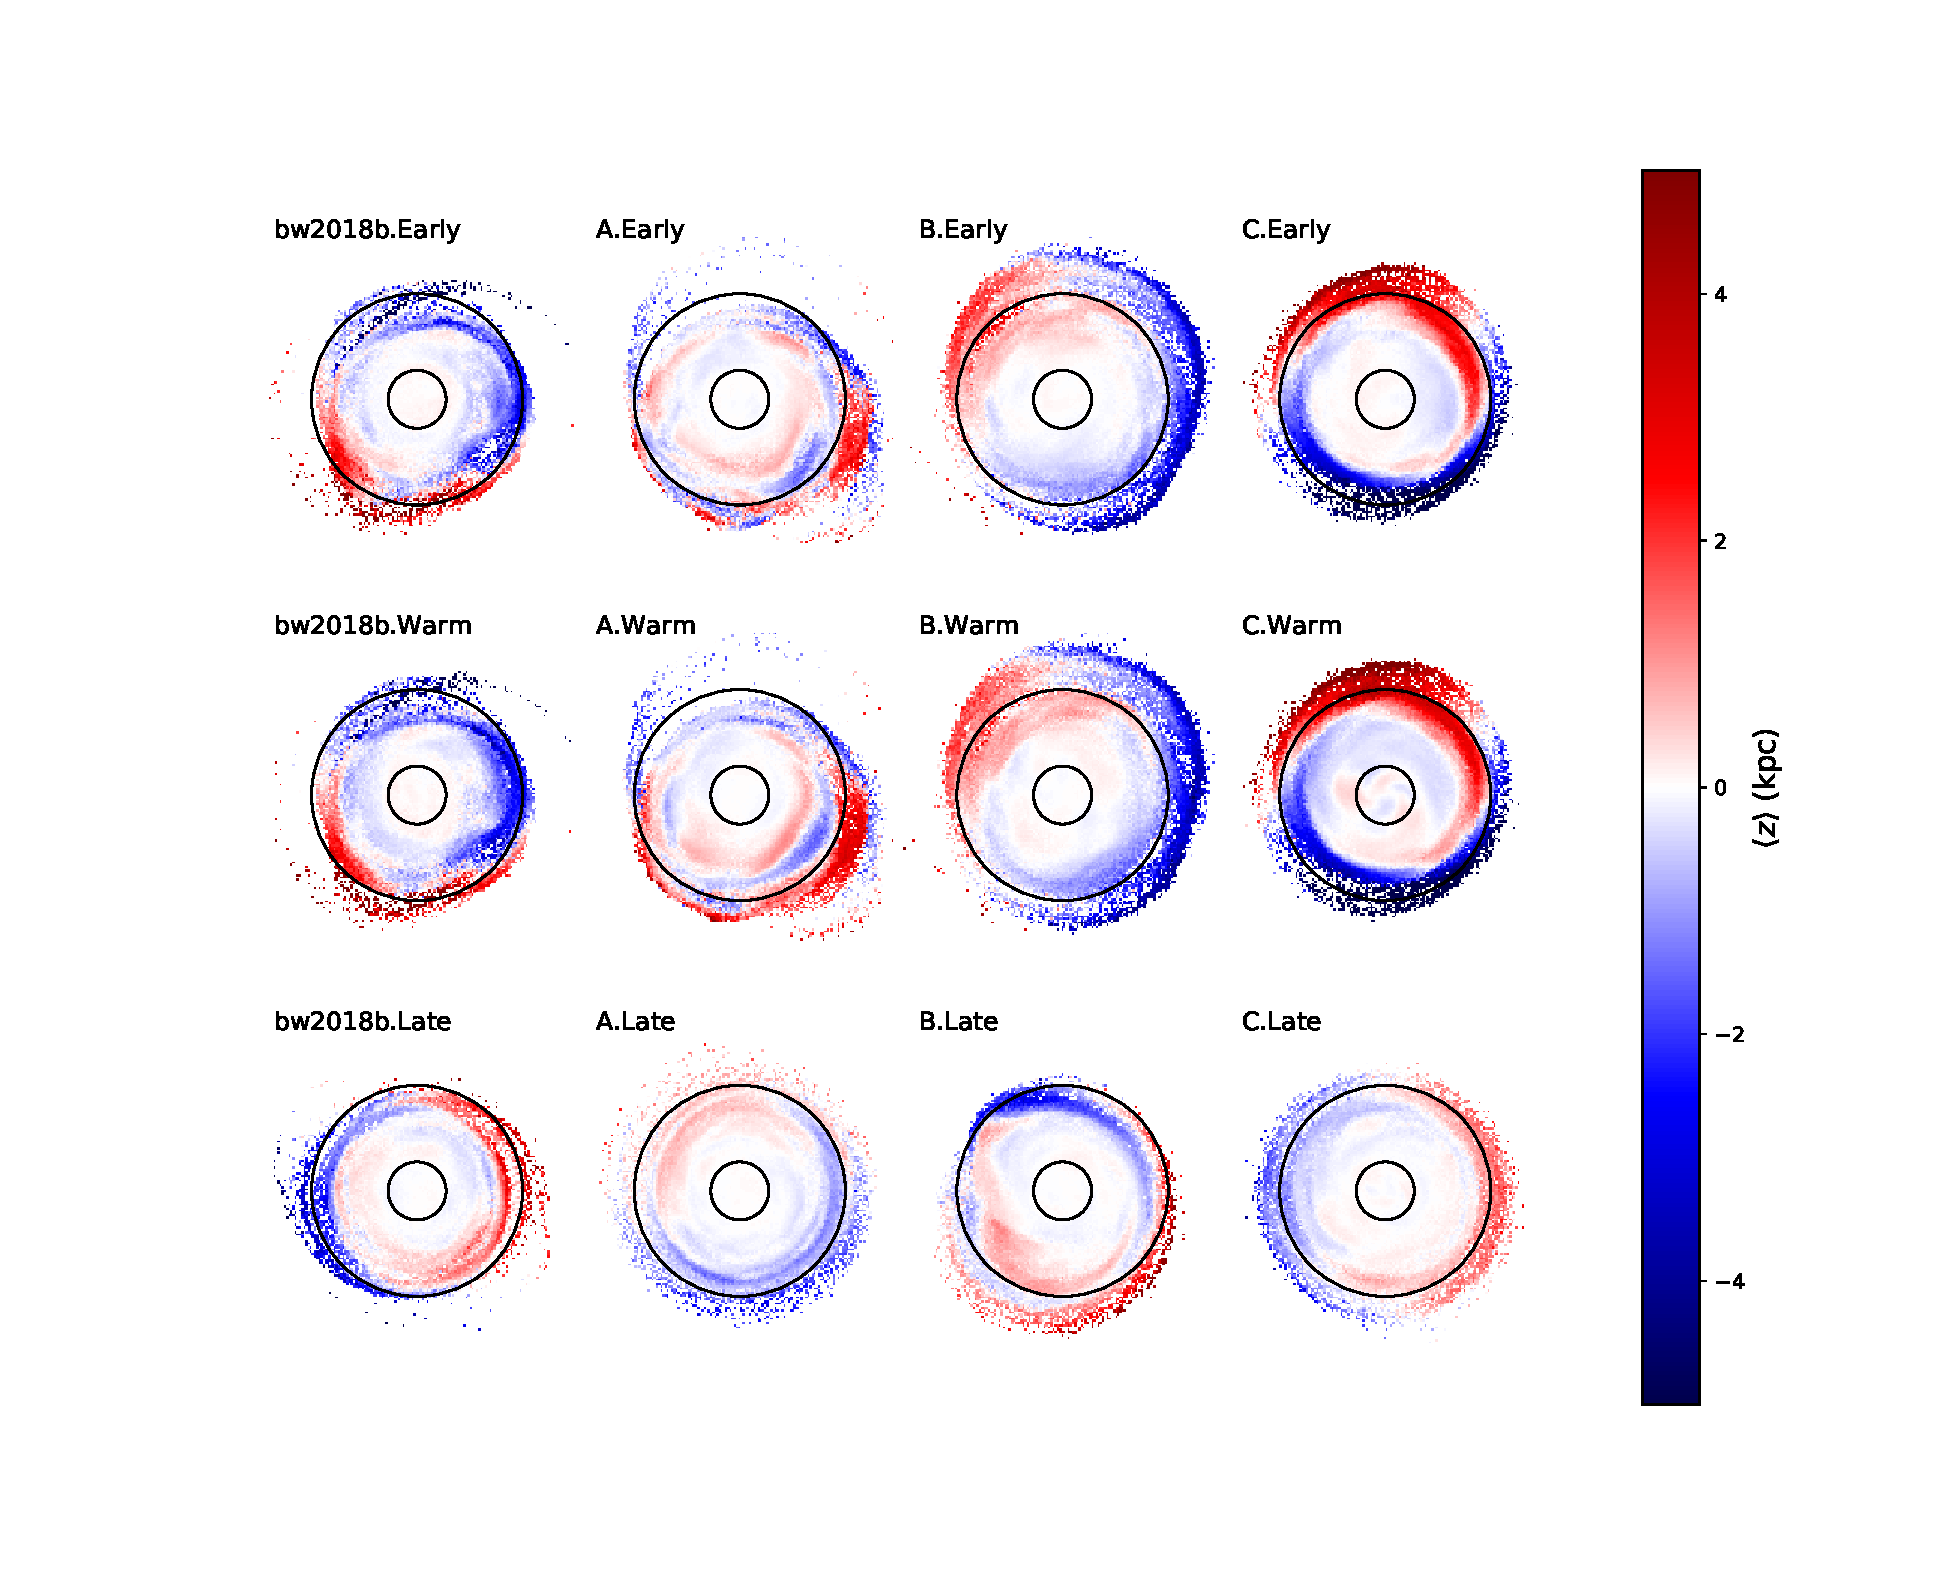
\includegraphics[width=0.8\textwidth]{../figures/twelve_panel_displacements_025.eps} \caption{Mean displacement above or below the disc at $a=0.625$ for the top two rows, and $a=0.875$ for the bottom row (late-insert suite). The circles correspond to $2.2 \,R_d = 8.1\,\kpc$ and $20 \, \kpch = 29.5\,\kpc$.  }
	\label{fig:vertical_displacement_map}
\end{figure}


\begin{figure}
	\centering
	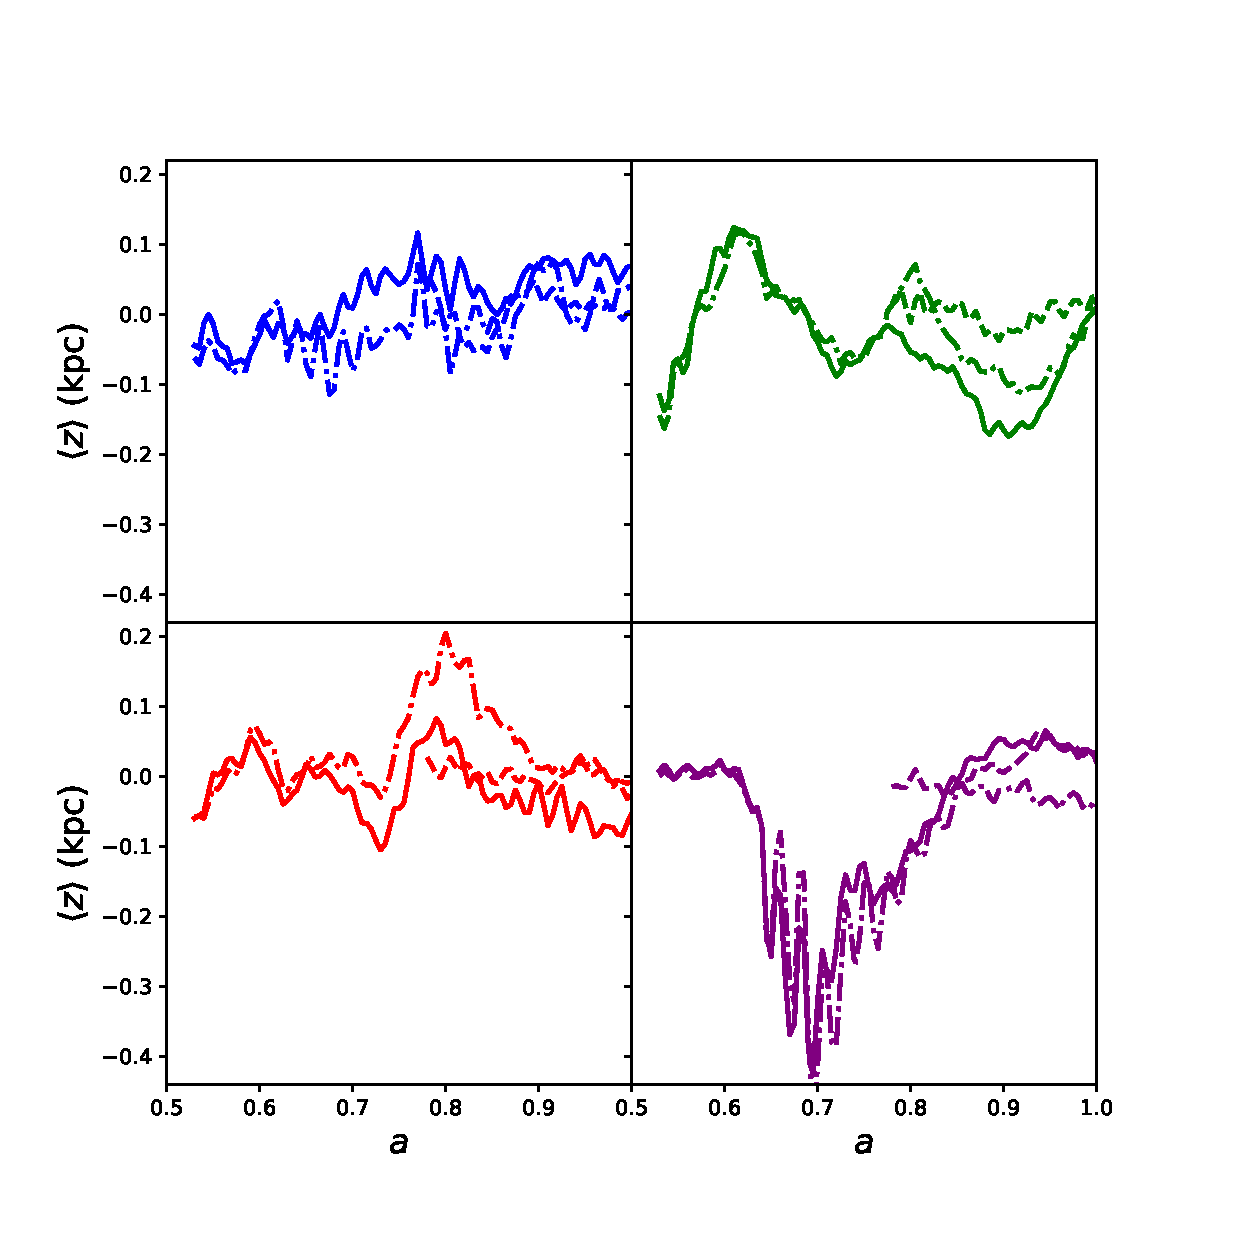
\includegraphics[width=0.8\textwidth]{../figures/z_0_all_models_four_panel.eps}
	\caption{The $m=0$ bending mode strength as measured by $Z_0(4.0 R_d < R < 4.5 R_d)$ as a function of time for all models. Colours are the same as in Fig. 5. Line types are Early (solid), Warm (dot-dashed), and Late (dashed).} \label{fig:z_0}
\end{figure}

\begin{figure}
	\centering
	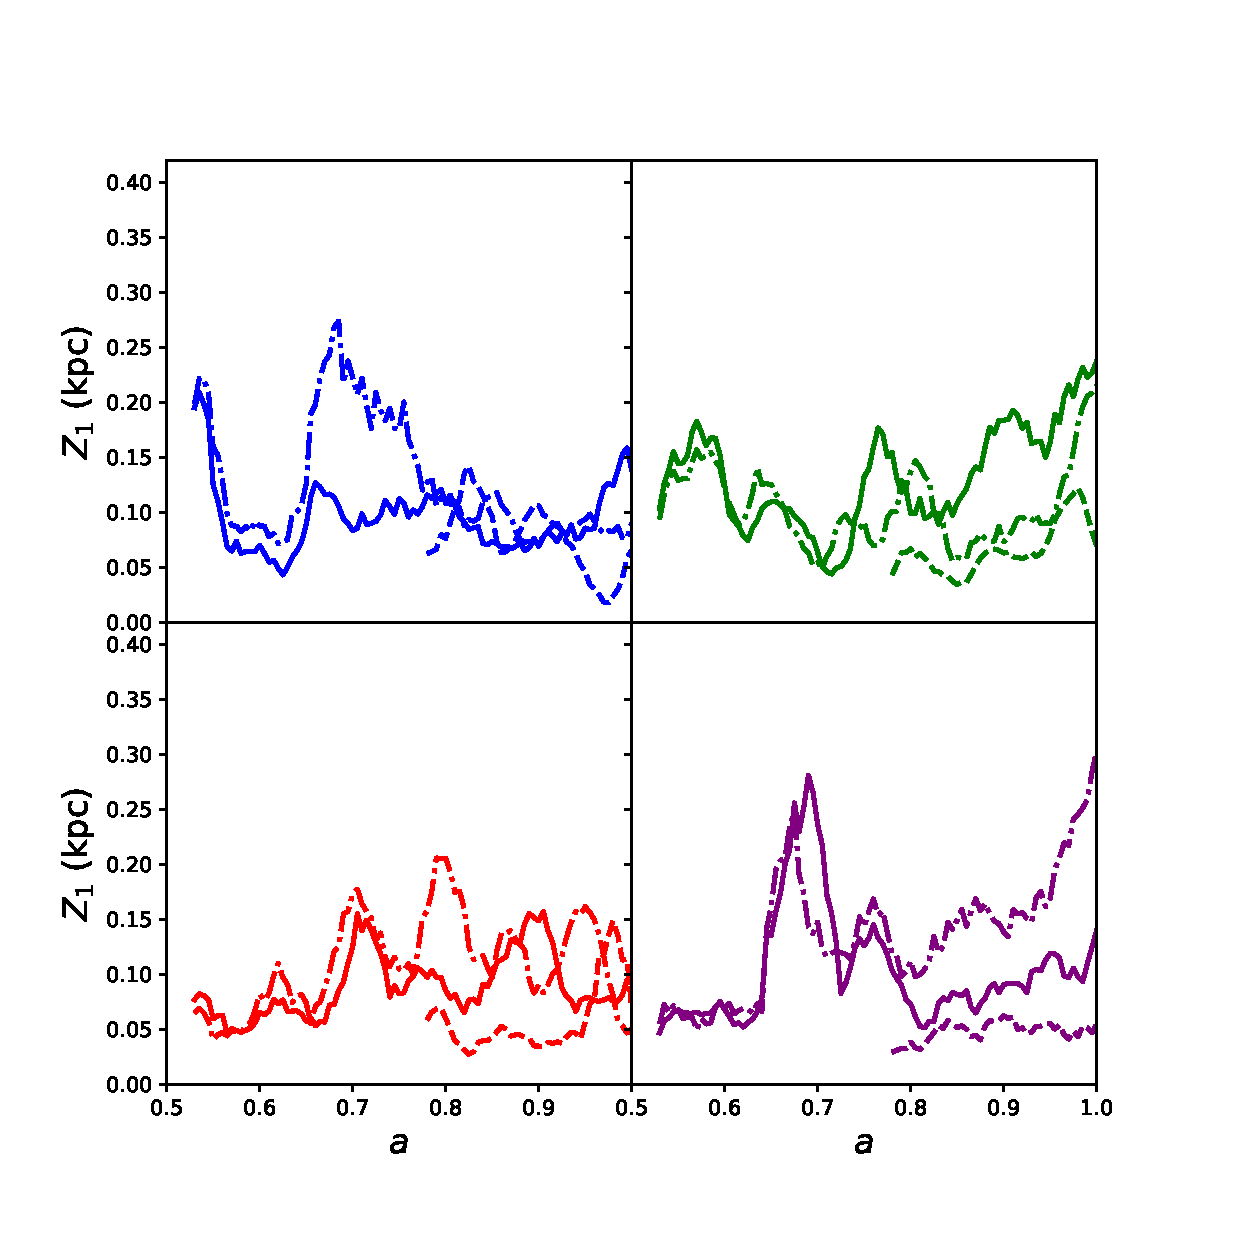
\includegraphics[width=0.8\textwidth]{../figures/z_1_all_models_four_panel.eps}
	\caption{The $m=1$ bending mode strength as measured by $Z_1(4.0 R_d < R < 4.5 R_d)$ as a function of time for all models. Colours are the same as in Fig. 5. Line types are Early (solid), Warm (dot-dashed), and Late (dashed).} \label{fig:z_1}
\end{figure}


We can get a feel for the various kinds of structure present in the disc by looking at the displacement maps in a single snapshot. Fig. \ref{fig:vertical_displacement_map} shows our models' mean height in the middle of their evolution. Substantial vertical structure is ubiquitous, with displacements growing in magnitude toward the outer disc. While $m=0$ structure is definitely present, the dominant mode in all cases appears to be $m=1$. Some simulations like A.Early and C.Warm appear to show higher-order bending structure as well. The suggestion is that cosmological discs cannot avoid forming substantial vertical structure, even in the quieter Late suite.

Fig. \ref{fig:z_0} shows the mean height in an approximately $2 \text{ kpc}$ annulus just beyond the solar neighborhood. A signal here represents a flapping mode of the disc that could appear as a Monoceros-like structure. The first thing we note is that the cases with the most halo misalignment, namely C.Early, show a very different flapping signature. C.Early displays a strong vertical displacement following bar buckling at $a=0.7$.  What separates C.Early from other simulations is that aside from this event, the disc does not flap over the simulation. In fact, C.Late has no distinguishable signal.

Aside from C.Early, all other discs immediately begin to flap on the scale of hundreds of parsecs. The most prominent example of this behaviour is seen in A.Early/Warm and B.Early/Warm. These simulations have distant massive substructures at initialization, possibly putting them on orbits with their substructures that induce flapping. Interestingly, the close encounter in B.Late produces far less flapping. A closer subhalo will displace the inner disc-halo system over smaller distances, which may explain why we do not see a strong $m=0$ signal in this case.

Aside from flapping modes, we might also observe Monoceros-like structures as rings of stars tilted from the disc. By computing $Z_1$ in this region, we can quantify this effect. All simulations see several hundred parsec $m=1$ bending modes in the region of Monoceros. Unlike flapping, $m=1$ bending modes appear to be more ubiquitous and have slightly higher magnitude. These bending modes also appear to be more sensitive to the initial dynamical temperature of the disc, with warmer discs generally producing stronger $m=1$ signal. We also note that where B.Late did not show any flapping from its substructure encounter, a 150 pc $m=1$ bending mode is observed following its massive subhalo's pericenter.

%\begin{equation}
%Z_m(S) = \left\vert \frac{1}{M_S} \sum_{j \in S} m_j z_j e^{i m \phi_j} \right\vert, \label{eq:z1}
%\end{equation}
%where $S$,$M_S$, and $\phi_j$ are defined as in Eq. \ref{eq:a2}, $z_j$ is the displacement of the $j$-th particle in $S$, and $m=1$ for the relevant bending mode. We take $S$ to be the annulus, $R \in [4.0 \,R_d,4.5\,R_d]$. The bending mode is plotted against time for all of our simulations in Fig. \ref{eq:z1}.  Milky Way discs are known to spontaneously form bending waves in isolation due to shot noise \citep{chequers_2017}, as well as in response to realistic populations of subhaloes \citep{chequers_2018}. In the absence of a major perturber, as in \citet{chequers_2018}, the $m=1$ height bending mode is constrained to less than but on the order of $10^{-1}$ in the region we are considering.

%In the top panel, the four simulations with the highest $m=1$ bending mode signals are bauer2018b.Early, bauer2018b.Warm, C.Early, and C.Warm. These simulations correspond to the most angularly displaced simulations in the entire suite. By contrast, bauer2018.Late, B.Early, B.Warm, and B.Late which only have satellite perturbers of Sgr mass have a peak signal on the order of half the angularly displaced simulations. The suggestion is that halo realignment causes stronger bending modes than a Sgr-like perturber would. This can be seen in Fig. \ref{fig:vertical_displacement_map} too, with the aforementioned simulations that are angularly displaced from their haloes showing kpc-scale perturbations in the region of Monoceros. It is also interesting to note that increased dynamical temperature does not suppress $m=1$ bending waves to any substantial degree, even in the quieter haloes.
%\subsection{Summary}

%Despite originating in moderately different halo environments, all models display qualitatively similar evolution. A bar begins to form almost immediately after the disc becomes live. The bar proceeds to buckle while vertical structure is excited through the disc, causing complicated vertical structure even in the disc interior. The bar grows and heats the disc, giving rise to something similar-looking present-day Milky Ways.


%Fig. XX shows the $v_z$ displacement field for all runs at select times.

%Fig. XX shows the correlation of $v_z$ and $z$ for all runs at select times.

%Fig. XX shows the strength of the $m=1$ modes for the three cylindrical velocity components vs time in all runs.

%Fig. XX shows the strength of the $m=2$ modes for the three cylindrical velocity components vs time in all runs.

\section{KUD Dynamics} \label{sec:kud}
In this section, we focus on stars which are stripped from the disc, and whose orbits take them to very high Galactic latitudes.
%The last section focused on bulk bending of the disc around the solar neighborhood. Here, we focus on stars which may be stripped from the disc to very high latitudes. We give a definition for this population and succinctly summarize its dynamics.

% Outer halo does not realign

% Discs that form early will be misaligned (Dubinski)



\subsection{Definition and Calculation from Simulations} \label{ssec:def}

\begin{figure}
    \centering
	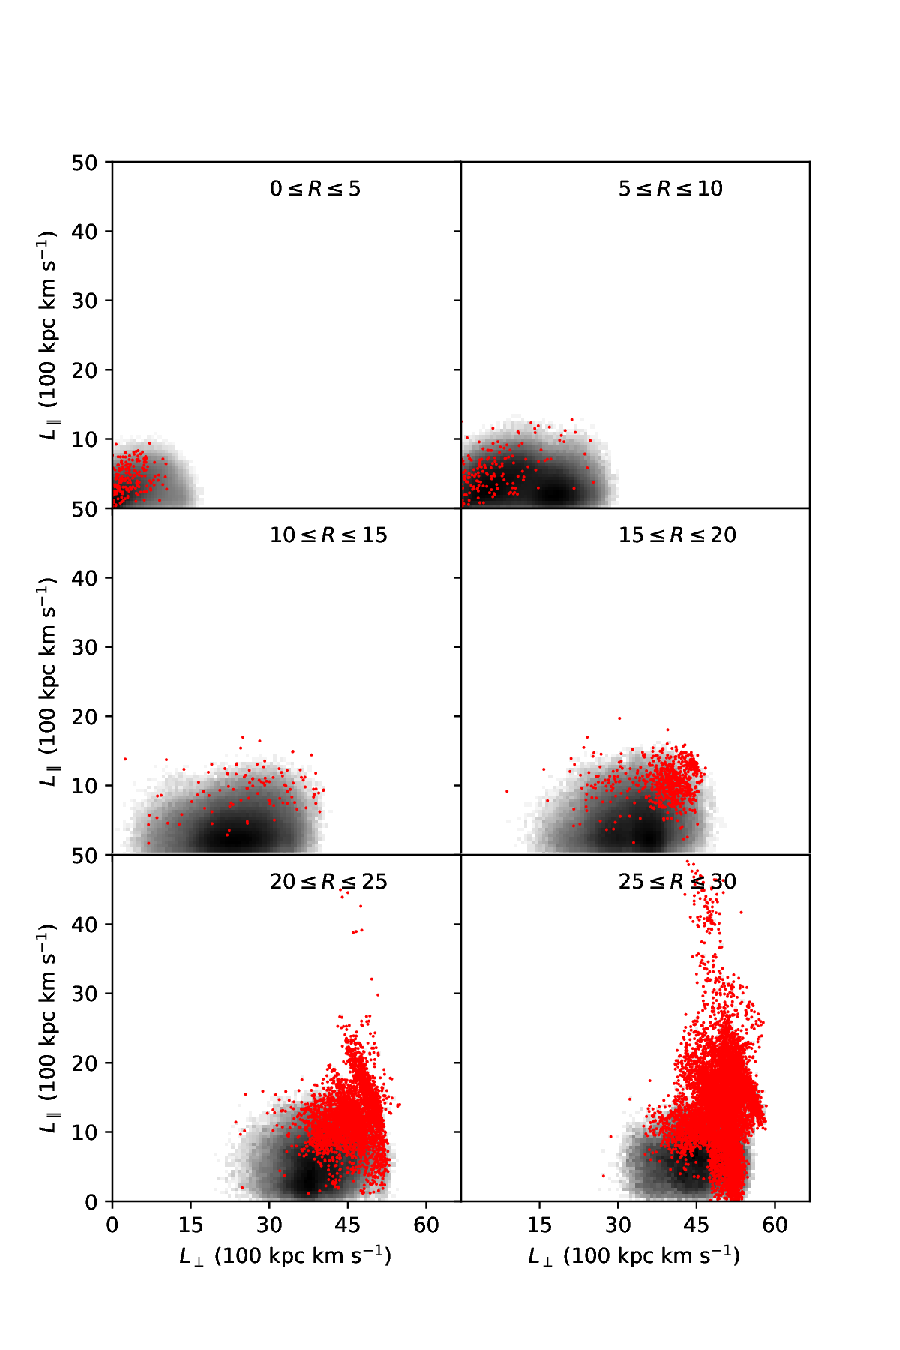
\includegraphics[width=0.8\textwidth]{../figures/angmom_268824_eta_8.pdf}
	\caption{A plot of KUD stars identified in red for $\eta=8$ in six spherical shells at present day. The shell limits are annotated in each panel. The smooth disc distribution is denoted by the histogram.}
	\label{fig:angmom_eta}
\end{figure}




\begin{figure}
    \centering
  	\subfloat[]{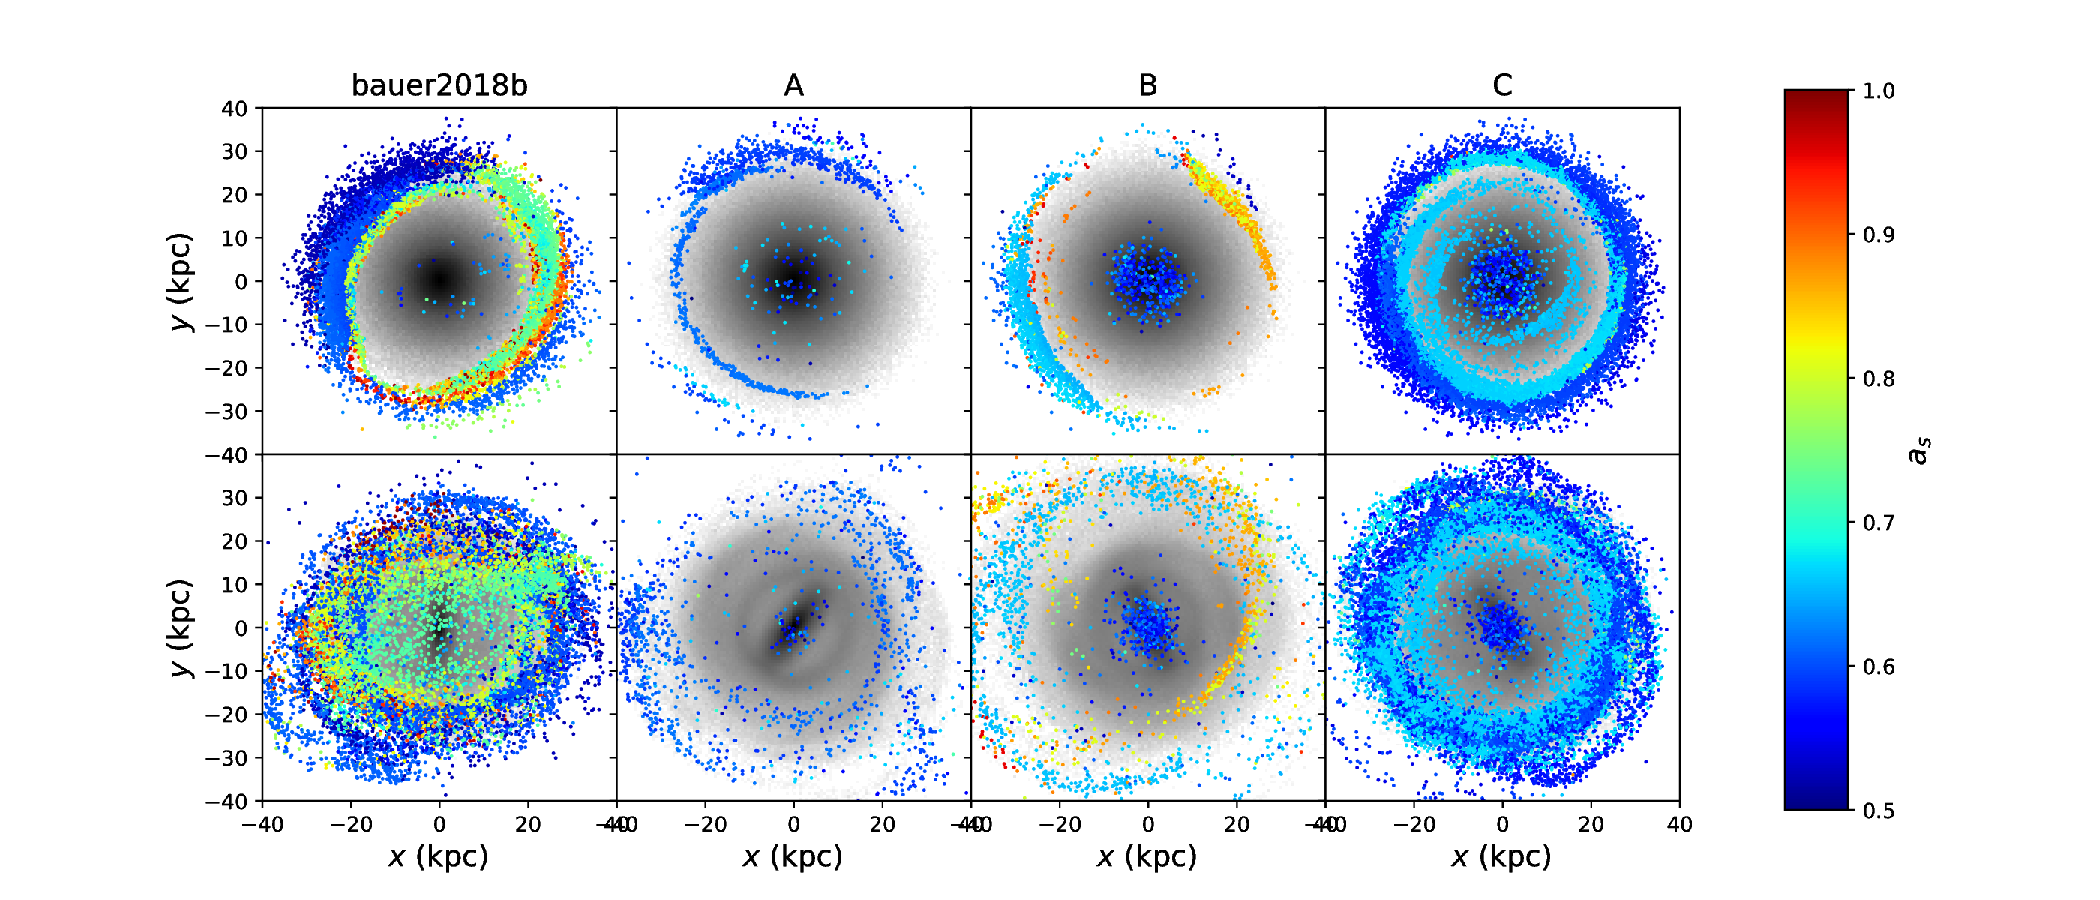
\includegraphics[width=0.8\textwidth]{../figures/kud_early_insert_face_on.pdf}}\\
	\subfloat[]{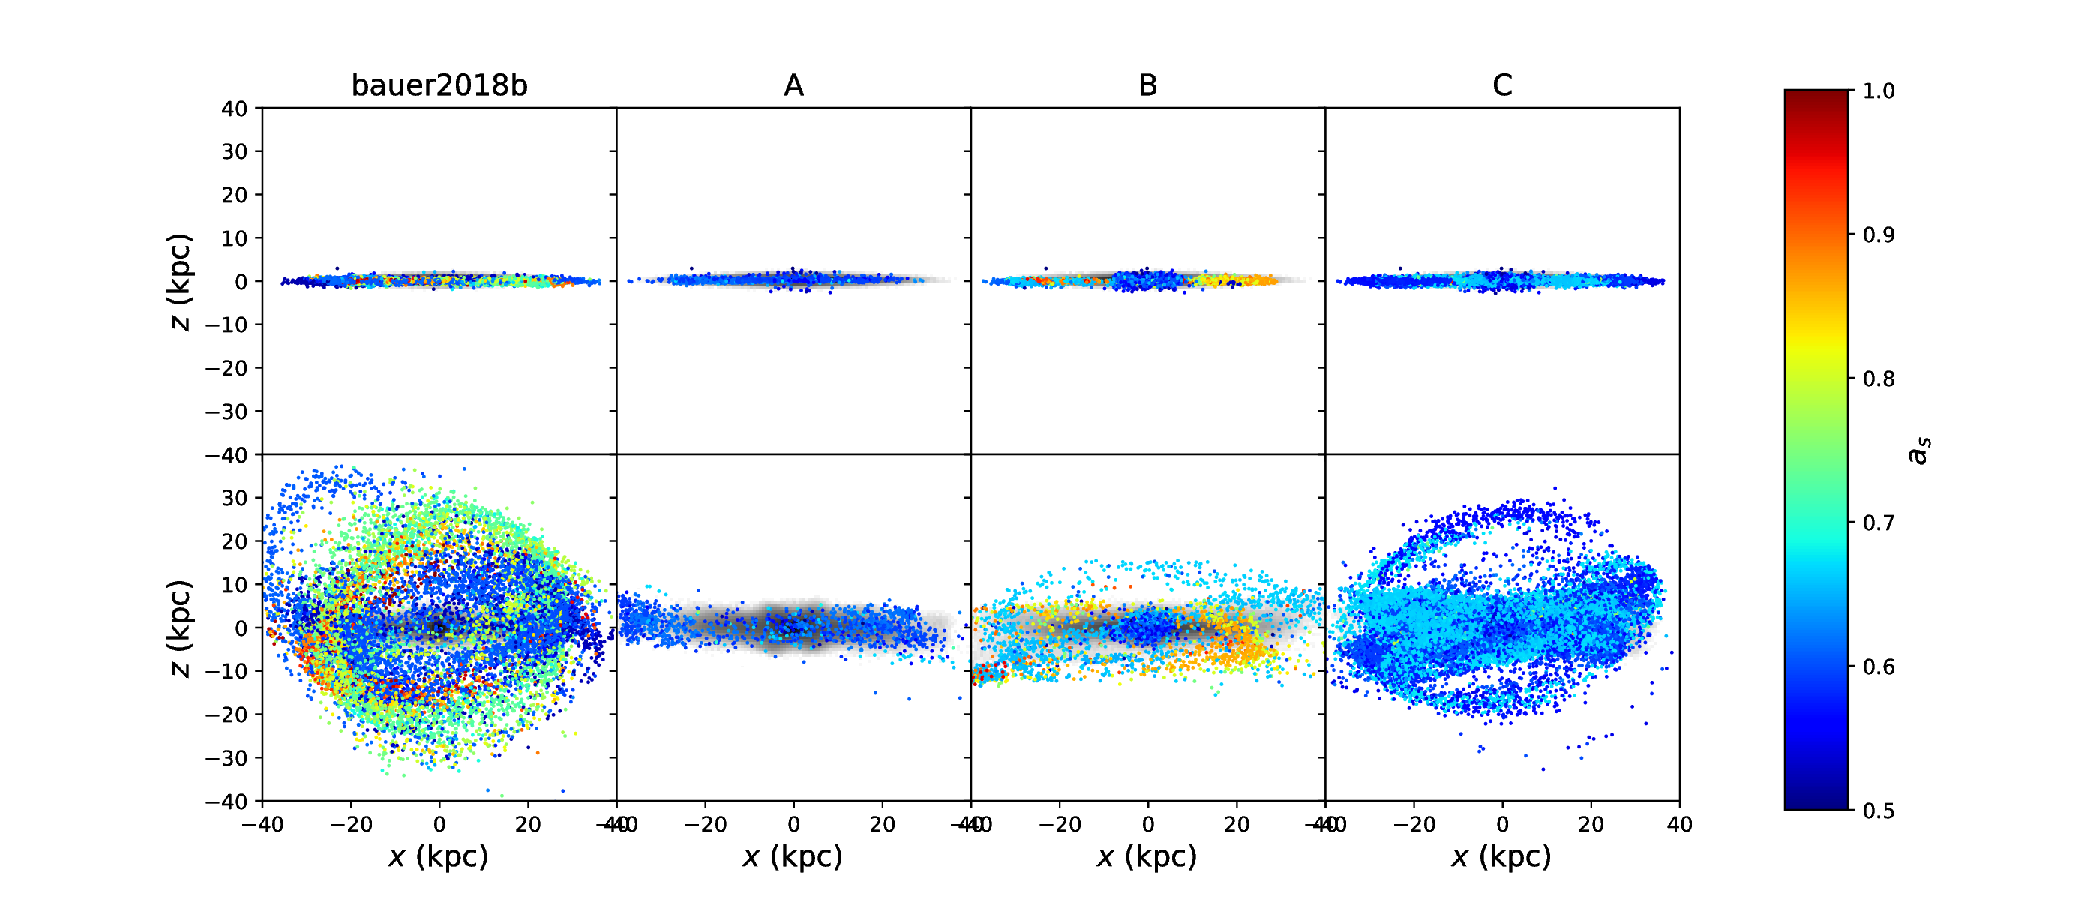
\includegraphics[width=0.8\textwidth]{../figures/kud_early_insert_edge_on.pdf}} \caption{KUD stars are shown for the fiducial suite in face-on (a) and edge-on (b) projections in the initial disc (upper panel) and final snapshot (lower panel). The non-kicked stars are shown as a histogram and the KUD stars are coloured by the time satisfying Eq. \ref{eq:kud_def}. Each column is one of the haloes considered in this paper.}
	\label{fig:kud_stars_final_ics}
\end{figure}
Any definition for what it means to be stripped from the disc is on some level arbitrary. Since we are interested in tracking a population of stars which reaches high Galactic latitudes, we simply set a height threshold for a stellar orbit. We then call a star kicked up at time $t_i$ for
\begin{equation}
t_{i} = \underset{t}{\operatorname{argmin}} \vert z_i(t) - \eta z_{rms}(R_p,t) \vert, \label{eq:kud_def}
\end{equation}
where $\eta$ is a free parameter, $t_{i}$ is the stripping time for the $i$-th particle, $z_i(t)$ is the height of the $i$-th particle in the body frame of the disc, interpolated between snapshots, and $z_{rms}(R_p,t)$ is the time-dependent $z_{rms}$ of the disc at an annulus centered on $R_p$. Expressed verbally, we identify KUD stars as those stars whose orbits take them a distance $\eta z_{rms}(R_p,t)$ from the midplane.


%\subsection{Choice of $\eta$} \label{ssec:choice}

The drawback to this definition is that observers only see a single snapshot of the Milky Way. To help observers identify the kinds of stars we are tagging, we present the following simplification. If we take the view of our disc being composed of two dynamical populations, KUD stars and planar disc stars, then the choice of $\eta$ tells us roughly how many exponential scale lengths above the disc we believe few in-plane disc stars exist. If the disc always has a uniform exponential scale height, $z_d$, then we expect $1.8\%$ to be above $4\,z_d$, $3.4 \times 10^{-2}\%$ to be above $8\,z_d$, and $6.1 \times 10^{-4}\%$ to be above $12 \,R_d$.

Furthermore, stars whose orbits stay in the plane of the disc will have large angular momentum components perpendicular to the plane. In the body frame, we say $L_\perp=L_z$ and $L_\parallel = \sqrt{L^2 - L_\perp^2}$, where $L$ is angular momentum magnitude for a star and $L_z$ is the component along the disc's spin axis. The stars which we identify as kicked up should be those which have relatively high $L_\parallel$ at some point in their evolution. 

Taking these things together, we take a look at how the choice of $\eta$ impacts the number of kicked-up disc stars identified in C.Early. Choices of $\eta=4$, $\eta=8$, and $\eta=12$ yield (216,529 particles, $6.2\%$), (18,612 particles, $5.3 \times 10^{-1}\%$), and (4,302 particles, $6.9 \times 10^{-2}\%$) KUD stars, respectively. In the cases of $\eta=8$ and $\eta=12$, the number of stars detected substantially exceeds the number expected from a smooth disc population assuming a uniform exponential scale length, by over an order of magnitude in each case. 
\begin{figure}
    \centering
  	%\subfloat[]{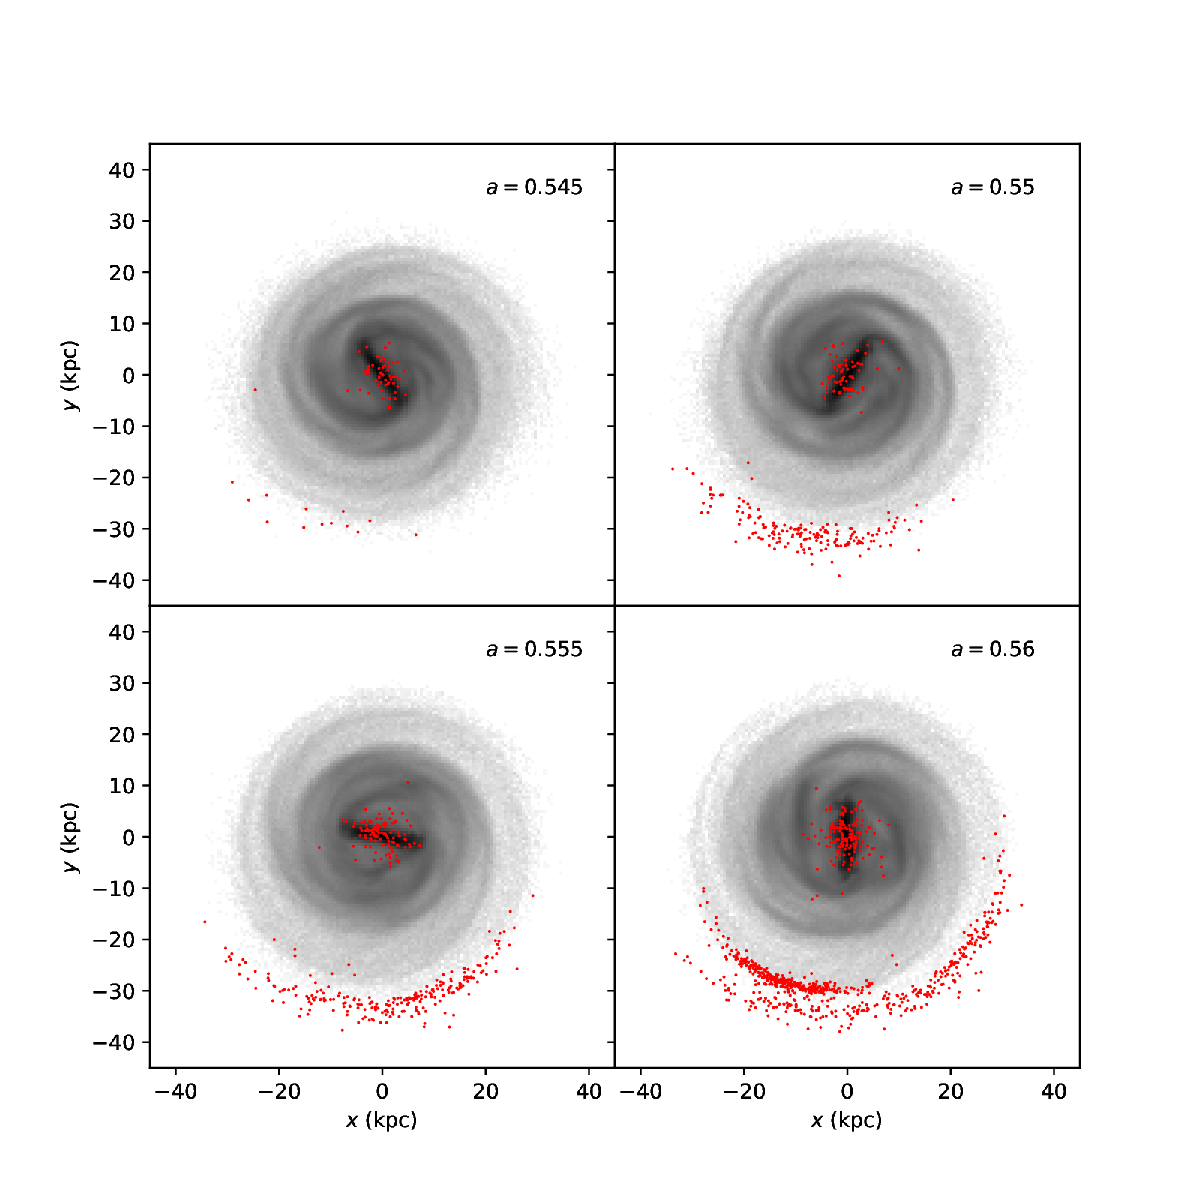
\includegraphics[width=0.45\textwidth]{../figures/fiducial_halo_268824_xy_s_009.pdf}}\\
	%\subfloat[]{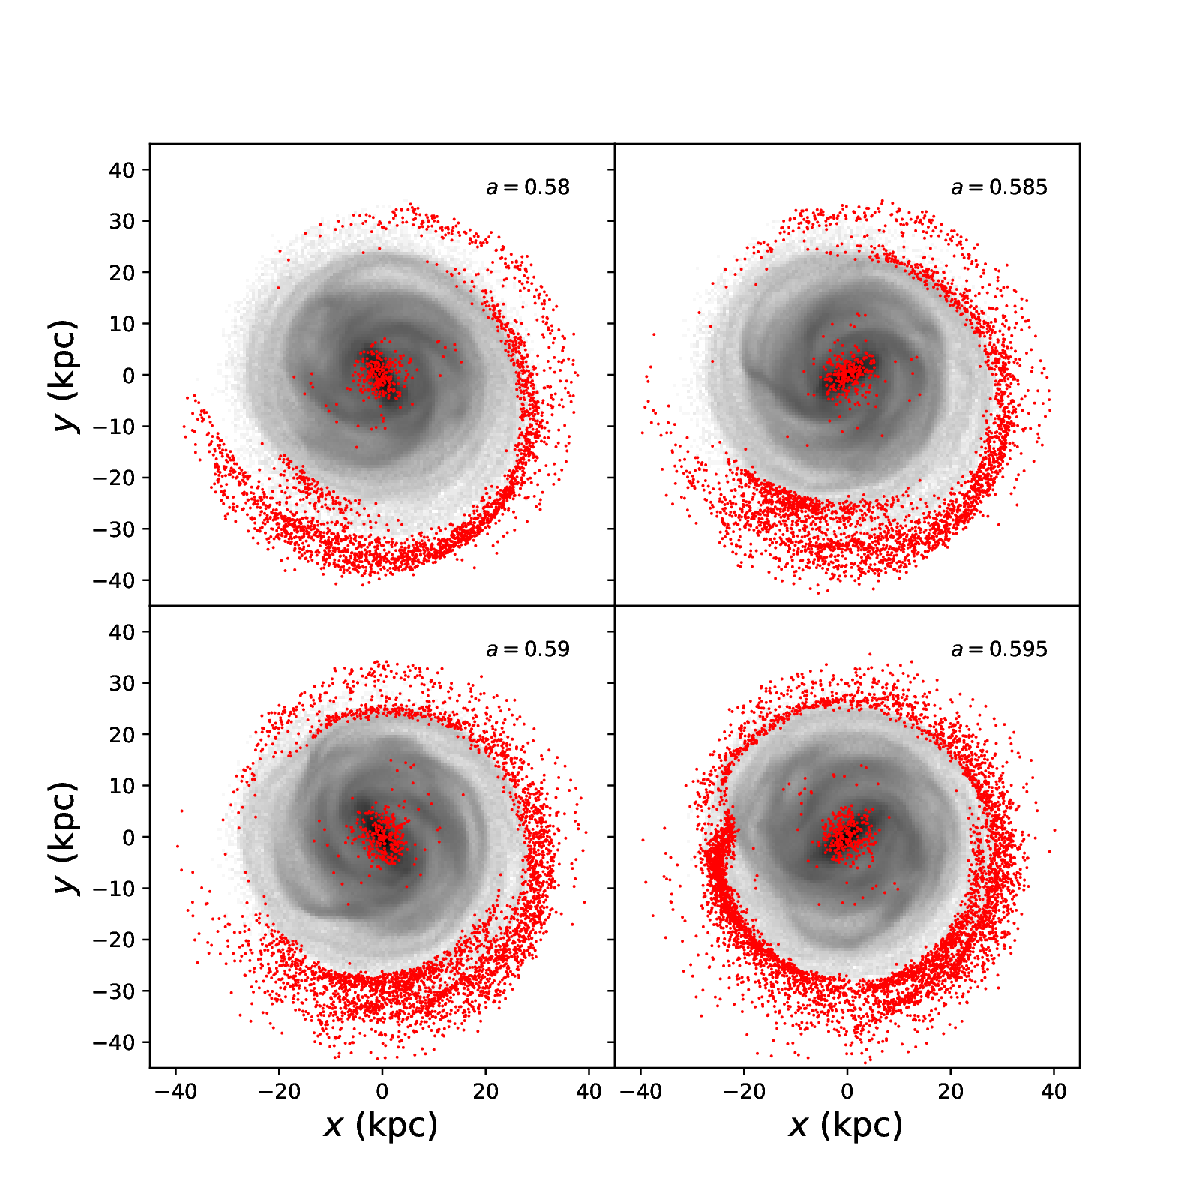
\includegraphics[width=0.45\textwidth]{../figures/fiducial_halo_268824_xy_s_016.pdf}} \caption{KUD stars are plotted for C.Early at the labeled times. The top panels (a) occur near the beginning of the simulation, before any KUD stars are generated, and the bottom panels (b) come slightly later. We see clear association with spiral arms, suggesting the same generation mechanism presented in \citet{laporte_2019_feathers}.}
	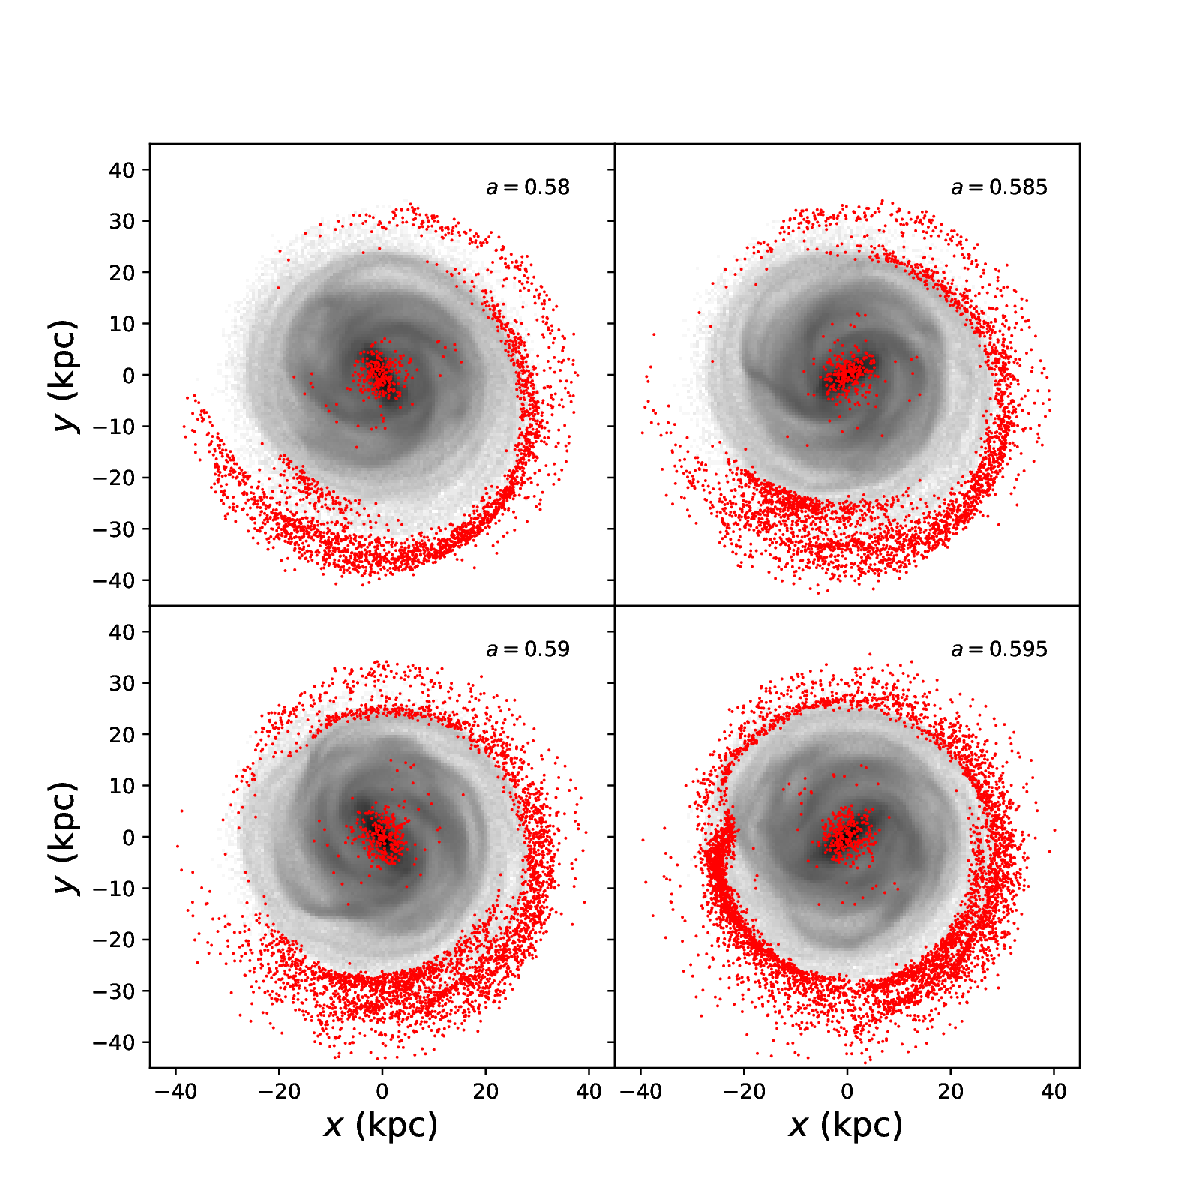
\includegraphics[width=0.8\textwidth]{../figures/fiducial_halo_268824_xy_s_016.pdf}
	\caption{KUD stars are plotted for C.Early at the labeled times. Note the association with spiral arms, suggesting a similar mechanism to \citet{laporte_2019_feathers}.}
	\label{fig:xy_tidal_tail_halo_c}
\end{figure}

\begin{figure}
    \centering
  	\subfloat[]{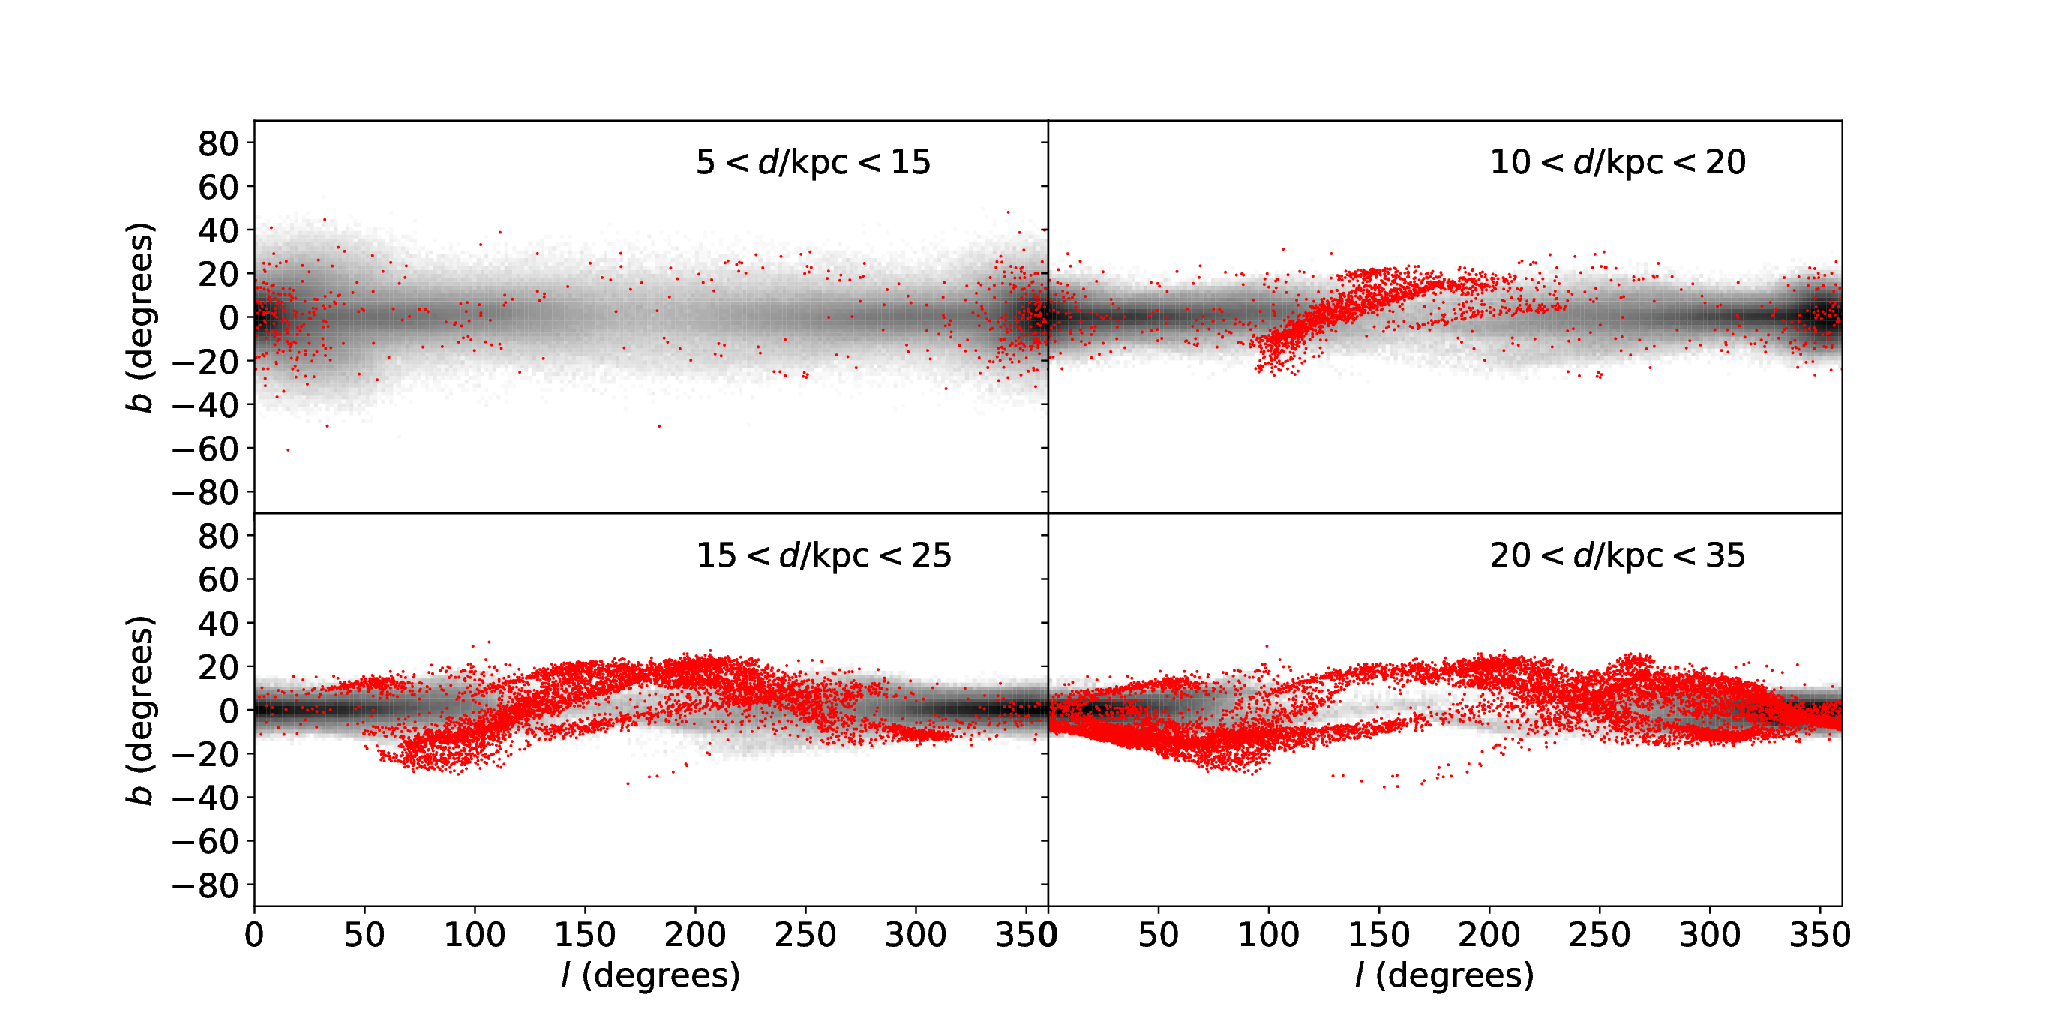
\includegraphics[width=0.8\textwidth]{../figures/fiducial_halo_268824_lb_s_055_overlay.pdf}\label{fig:lb_halo_c_warm_comparison}}\\
  	\subfloat[]{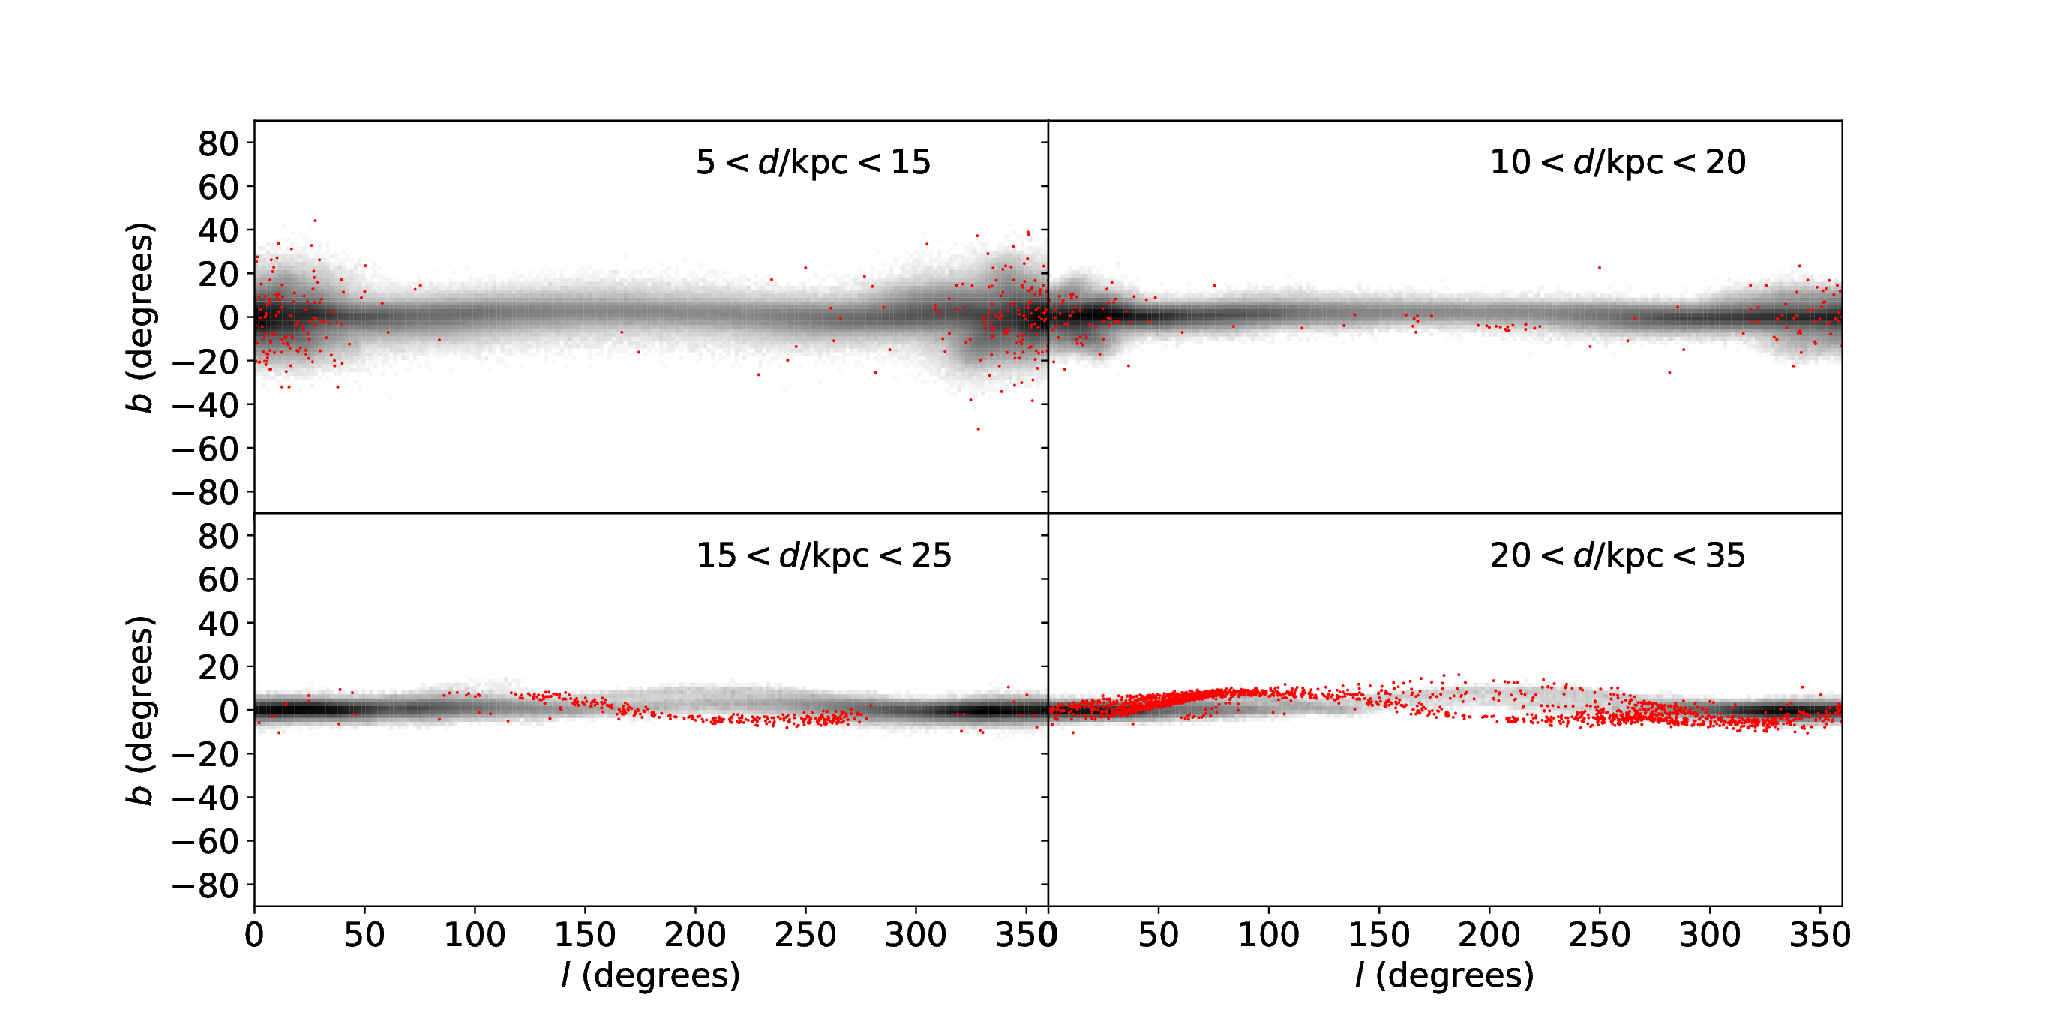
\includegraphics[width=0.8\textwidth]{../figures/fiducial_halo_268818_late_insert_lb_s_095_overlay.pdf} \label{fig:lb_halo_b_late}}
	%\subfloat[]{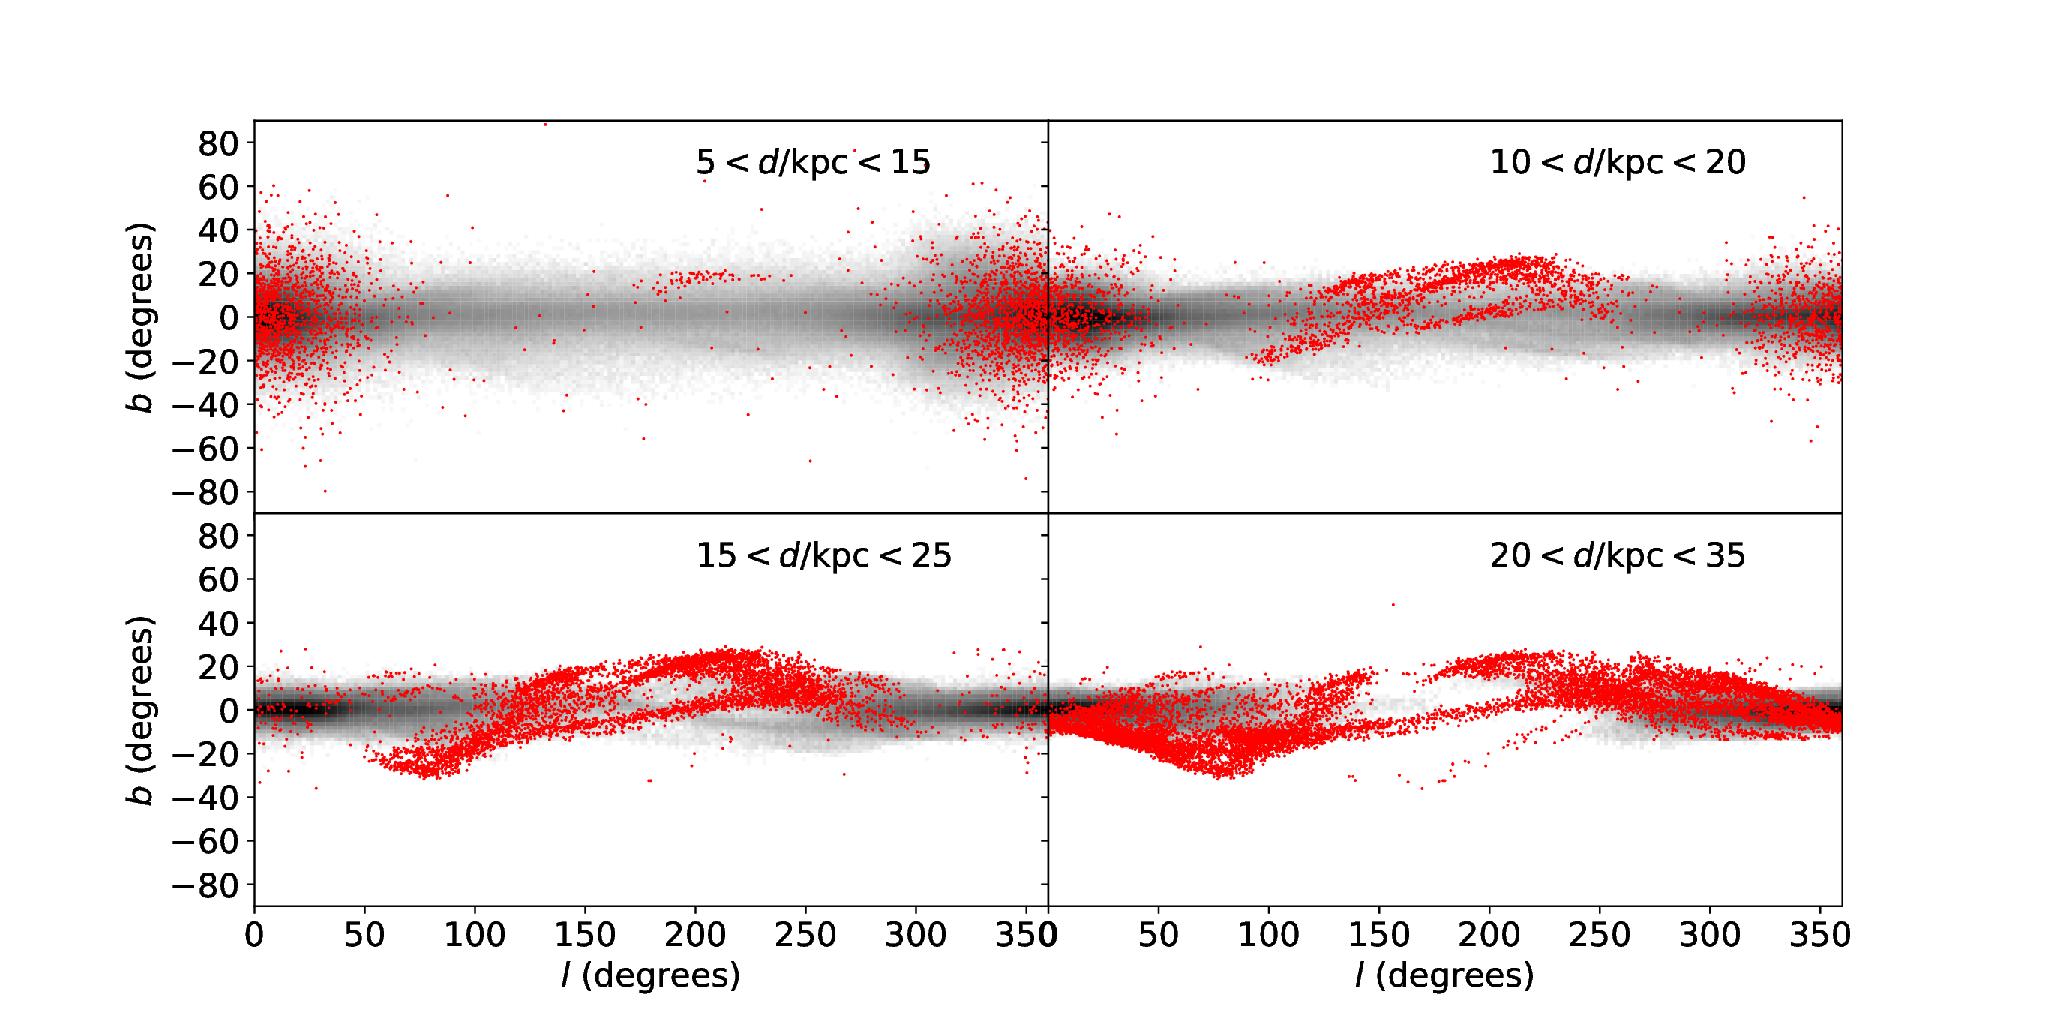
\includegraphics[width=0.45\textwidth]{../figures/fiducial_halo_268824_warm_lb_s_055_overlay.pdf}} 
	\caption{Heliocentric views of KUD stars in several different distance shells. The top panel depicts this for C.Early at $a=0.775$. The bottom panel shows the same for B.Late at $a=0.975$.}
\end{figure}


\begin{figure}
	%\subfloat[]{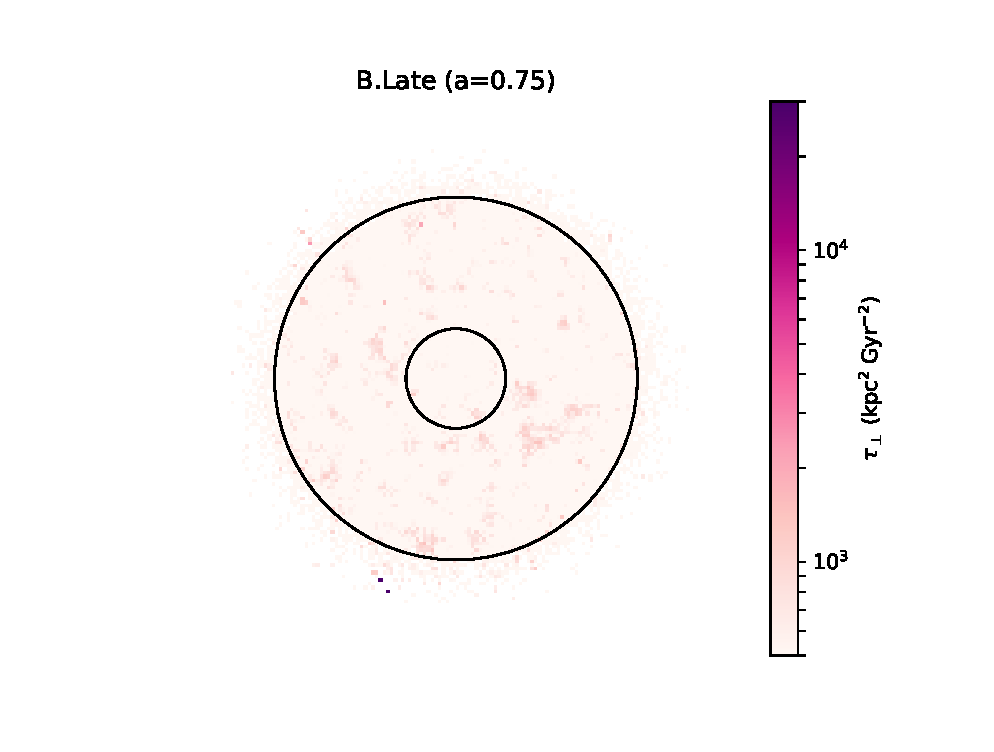
\includegraphics[width=0.45\textwidth]{../figures/b_late_torque_a_0_75.eps}}\\
	%\subfloat[]{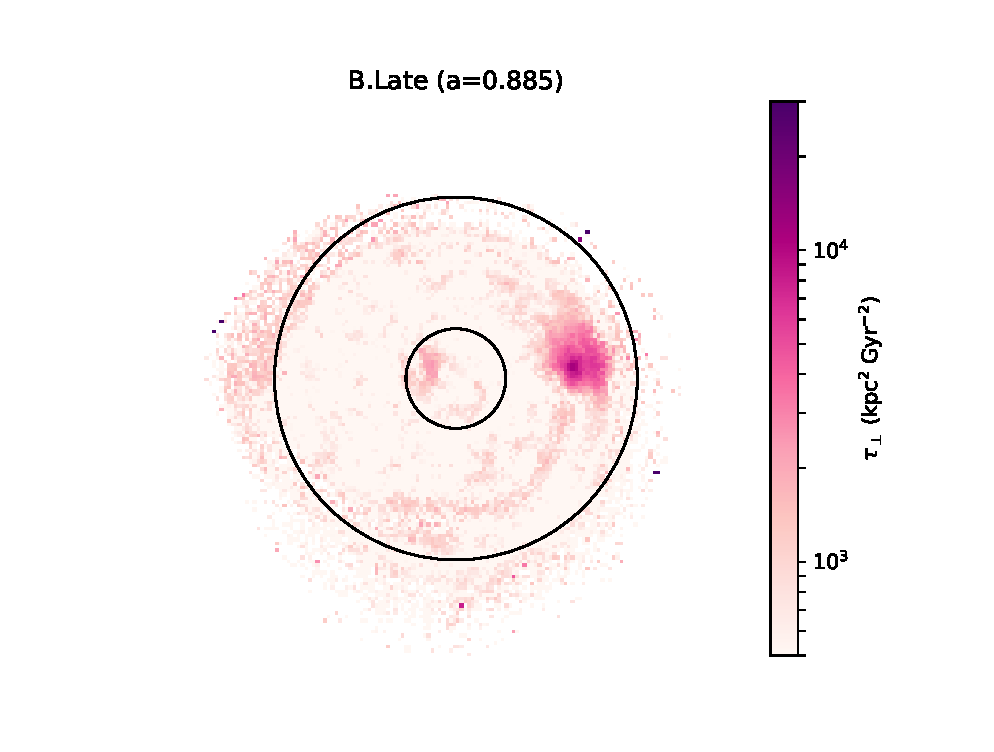
\includegraphics[width=0.45\textwidth]{../figures/b_late_torque_a_0_885.eps}}
	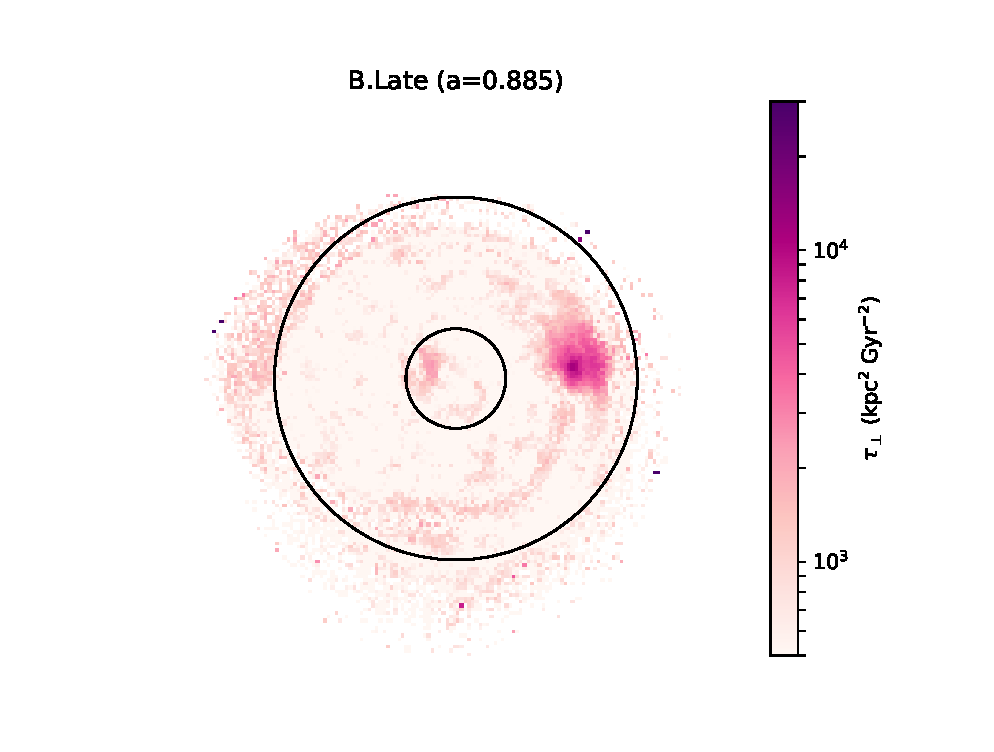
\includegraphics[width=0.8\textwidth]{../figures/b_late_torque_a_0_885.eps}
	%\caption{The $x-y$ projected perpendicular torques on the disc in B.Late at two different snapshots. The first is at initialization, and the second is when the most massive substructure in B.Late is at pericentre. The circles correspond to $R_p = 2.2\,R_d=8.1\,\kpc$ and $20\,\kpch=29.5\,\kpc$.}
	\caption{The $x-y$ projected perpendicular torque on the disc in B.Late at $a=0.885$. This corresponds to when the most massive substructure in B.Late is at pericentre. The circles correspond to $R_p = 2.2\,R_d=8.1\,\kpc$ and $20\,\kpch=29.5\,\kpc$.}\label{fig:torque_b_late}
\end{figure}


\begin{figure}
	\centering
	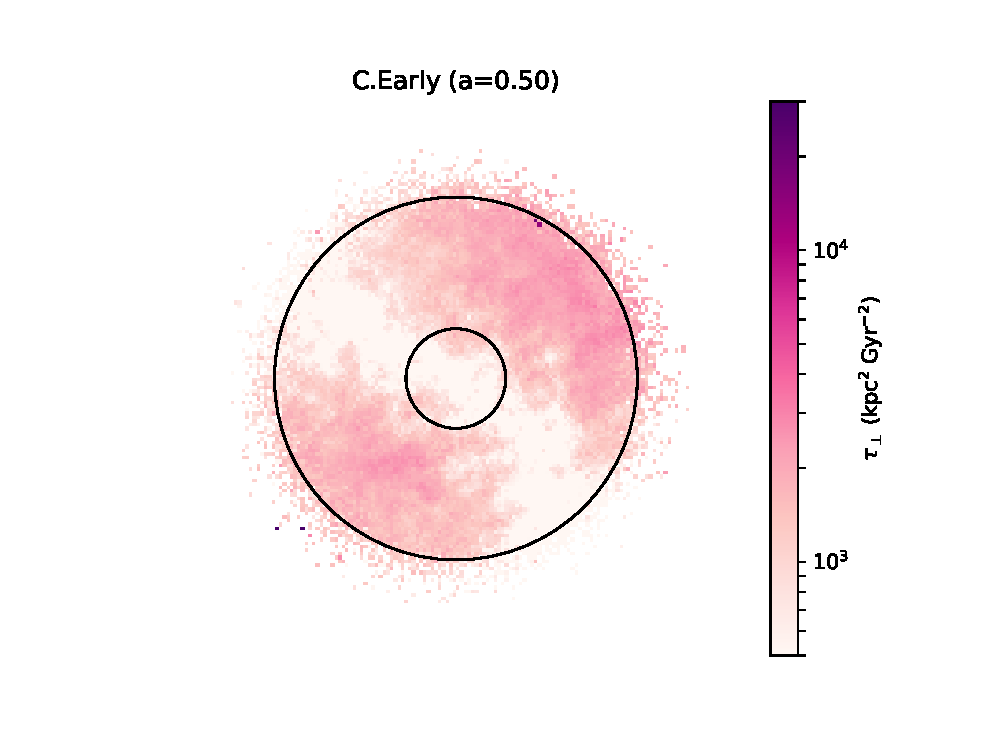
\includegraphics[width=0.8\textwidth]{../figures/c_early_torque_a_0_5.eps}
	\caption{Same as Fig. \ref{fig:torque_b_late}, but for C.Early at initialization ($a=0.50$).} \label{fig:torque_c_early}
\end{figure}
\begin{figure}
	\centering
	\subfloat[]{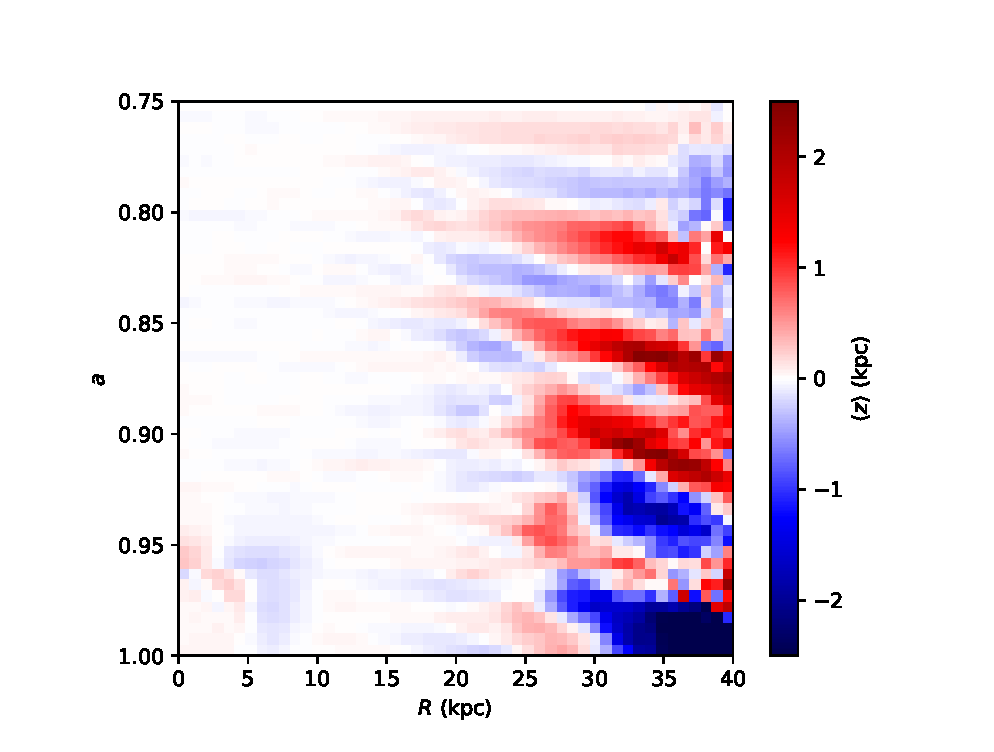
\includegraphics[width=0.45\textwidth]{../figures/b_late_z_0_r_a.eps} \label{fig:b_late_r_a}}
	\subfloat[]{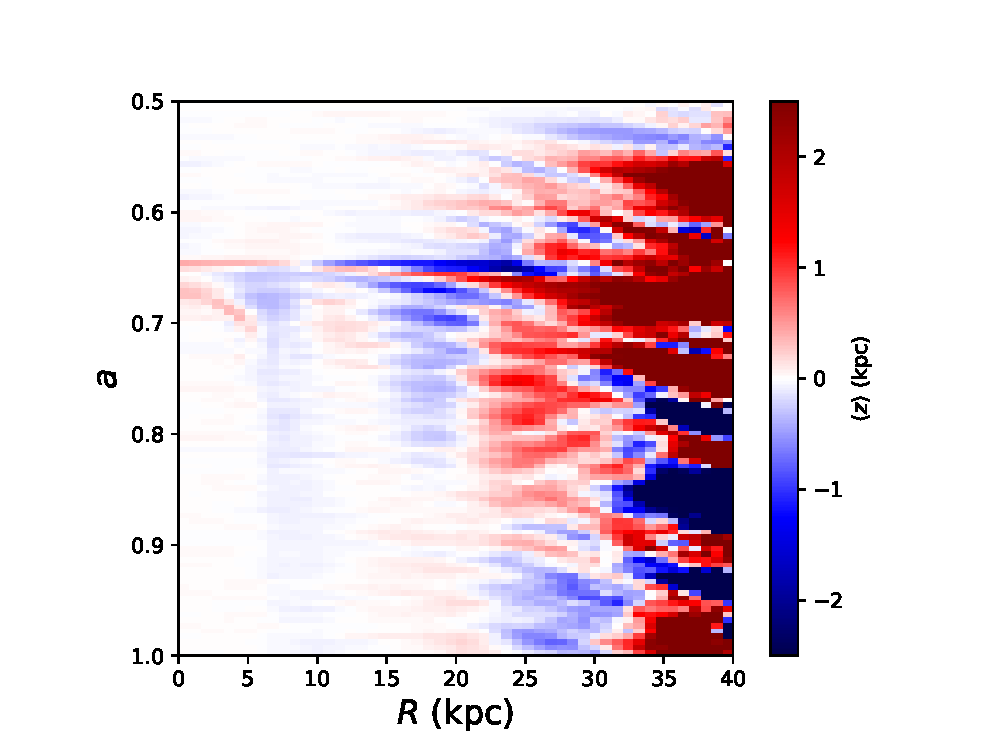
\includegraphics[width=0.45\textwidth]{../figures/c_early_z_0_r_a.eps} \label{fig:c_early_r_a}}\\
	\subfloat[]{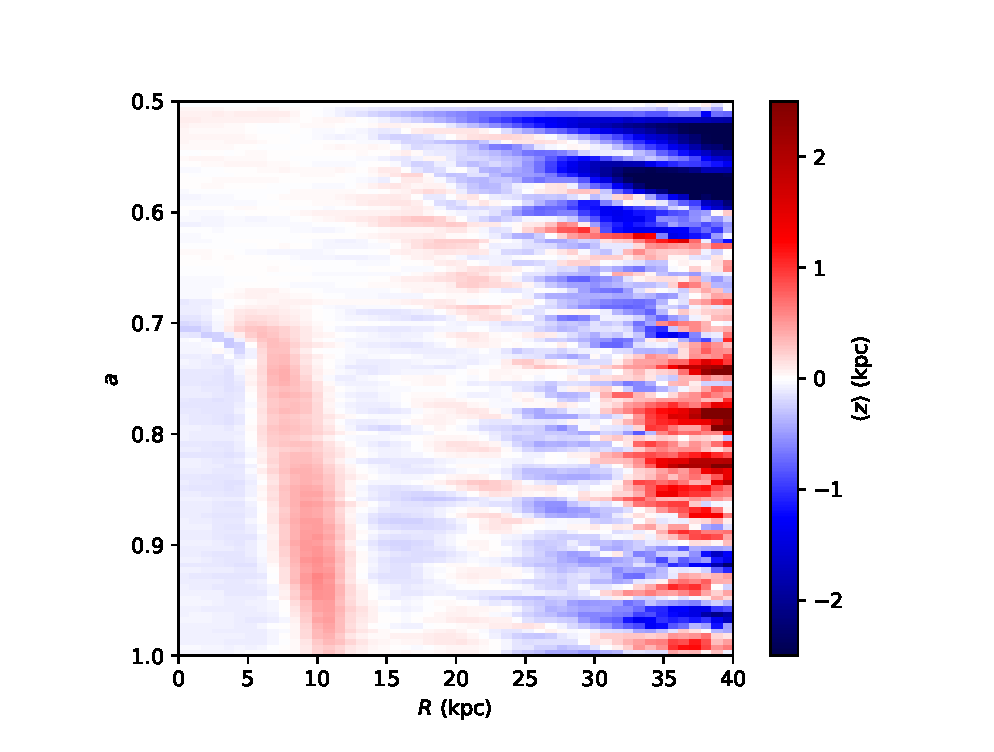
\includegraphics[width=0.45\textwidth]{../figures/a_early_z_0_r_a.eps} \label{fig:a_early_r_a}}	\caption{The $m=0$ bending mode for B.Late (a), C.Early (b), and A.Early (c) as a function of radius and scale factor. }
\end{figure}

For a choice of $\eta=8$, we have Fig. \ref{fig:angmom_eta} showing the angular momentum decomposition of the KUD stars in spherical shells in relation to the smooth disc. As expected, the stars that are identified here have high $\L_\parallel$ in general, except at high radii where high $L_\perp$ stars may still be identified as KUD stars with our definition. It is likely that there is some contamination at these radii by stars which were simply part of a warp, but this is to be expected for our simplistic definition.


\subsection{KUD Star Dynamics} \label{ssec:kud_dynamics}


We now turn our attention to the dynamics of the stars identified with our choice of $\eta=8$. Fig. \ref{fig:kud_stars_final_ics} shows the KUD stars in our fiducial suite in two different projections in both the final snapshot and initial conditions. Specifically, the top rows of (a) and (b)  show all of the stars kicked up by the the end of the simulation rewound  to where they come from in the initial disc.  The bottom rows show where they are in the final snapshot.

On one extreme, A.Early shows very little KUD structure, and the KUD structure it does have exists at very low latitudes, kicked up very early in the simulation. B.Early forms a few small streams at times we know it has a close encounter with a massive subhalo. We note the discrete groups of kick-up times in this simulation. 
The two plotted simulations that show substantial KUD populations are bauer2018b.Early and C.Early. These also correspond to the most misaligned halo environments with short $T_\tau$. In both cases, we see a continuous range of times over which stars are excited, rather than discrete events. Furthermore, in the case of C.Early, it seems like some stars are transported from the inner disc to form part of the kicked up population.





The mechanism in C.Early by which stars from the inner disc can be kicked up is highlighted in Fig. \ref{fig:xy_tidal_tail_halo_c}. Each new round of KUD stars appears to be associated with a wrapping spiral pattern. Together with Fig. \ref{fig:kud_stars_final_ics}, we are left  with the picture that  KUD stars generally come from the outer disc. In some environments, like in C.Early, strong spiral structure transfers stars outward and into strong warps. Some stars in these warps are stripped from the disc entirely. The stripped stars then phase mix to form the high-latitude structures seen in the final snapshot of C.Early.


\citet{laporte_2019_feathers} shows what the tidal arm transport mechanism looks like from the position of the Sun. Stars associated with the tidal tails seen in Fig. \ref{fig:xy_tidal_tail_halo_c} form filamentary structures with a characteristic bifurcation. They call the bifurcated parts of these structures ``feathers". A feather is visually identified after the fact, and like our KUD star definition, is an arbitrary delineation.

In  Fig. \ref{fig:lb_halo_c_warm_comparison}, we see the KUD stars in C.Early as they appear from the Solar neighborhood at $a=0.775$. The stars form the top and bottom feather structure described in \citet{laporte_2019_feathers}, and are undoubtedly associated with grand design spiral structure. The similarities suggest that global tides, at least superficially, create observable, stream-like structures at low-to-mid Galactic latitudes, extending along the length of the sky.


We contrast this to the moderate-mass Sgr interaction presented in B.Late. From the perspective of the Sun, we can look at the KUD structure present in B.Late, shown in Fig. \ref{fig:lb_halo_b_late}. The stars in this simulation that are identified as kicked up appear at relatively low latitudes overall, consistent with the idea that even a moderate mass Sgr dSph could not excite high latitude structures on a small timescale. 




\section{What Causes the Milky Way's Vertical Structure?} \label{sec:disentangle}

In this section, we delve into more detail regarding potential observational signatures in the vertical structure of stellar discs that would delineate between different environments. 





\subsection{Torque Signature from Halo Environments} \label{ssec:torque_signature}


We return to our choice cases here, and study their evolution in more detail. First, we want to understand the relevant torques in our models. We first look at B.Late, our Sgr dSph interaction analogue. The torque is measured at $a=0.885$ in Fig. \ref{fig:torque_b_late}, when the first pericentre occurs at around $R = 30 \,\kpc$. An interesting feature of the torque at the pericentric passage is that it does not have $m=2$ symmetry. There is no smooth torque pattern outside the off-center interaction pattern from the substructure.

The torque signature of the purely misaligned environment is very different from the satellite infall scenario. We plot the torque at initialization for C.Early in Fig. \ref{fig:torque_c_early}. Instead of presenting an asymmetric $\tau_\perp$ at a substructure pericenter, C.Early presents am $m=2$ symmetric torque which diminishes with decreasing radius. The torque magnitude is slightly lower than Fig. \ref{fig:torque_b_late} overall, but persists in future snapshots not presented here. It is worth mentioning that this simulation sees a continuum of times in which KUD stars are produced.

The takeaway here is that a halo misalignment produces $\tau_\perp$ slightly less than in a massive satellite encounter, but that the consistent exposure over a billions of years at the beginning of the simulation can cause more drastic KUD behavior in a continually excited fashion, rather than simply at each pericentric passage of a satellite. The presence of low-latitude streams cannot be a unique signature of a massive satellite interaction, as we will discuss.
 
\subsection{Time Evolution in Characteristic Scenarios} \label{ssec:mean_height}
\begin{figure}
	\centering
	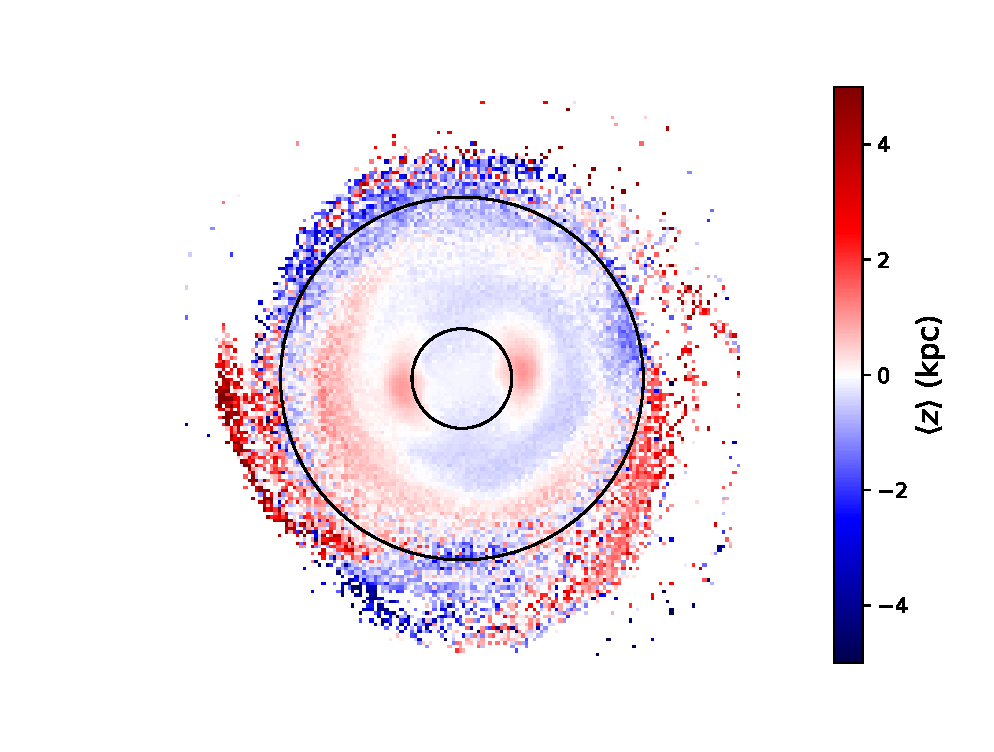
\includegraphics[width=0.8\textwidth]{../figures/a_early_displacement_a_0_875.eps}
	\caption{The mean height, $\langle z \rangle$, map for A.Early at $a=0.875$.}\label{fig:a_early_displacement}
\end{figure}








\begin{figure}
	\centering
	\subfloat[]{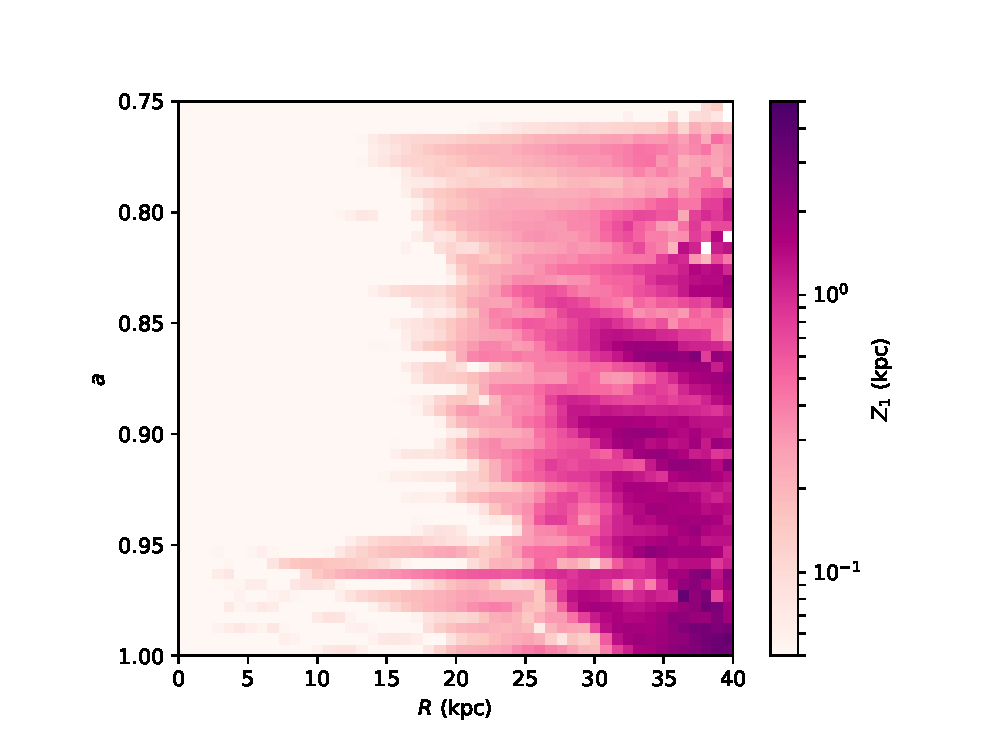
\includegraphics[width=0.45\textwidth]{../figures/b_late_z_1_r_a.eps} \label{fig:b_late_r_a_1}}
	\subfloat[]{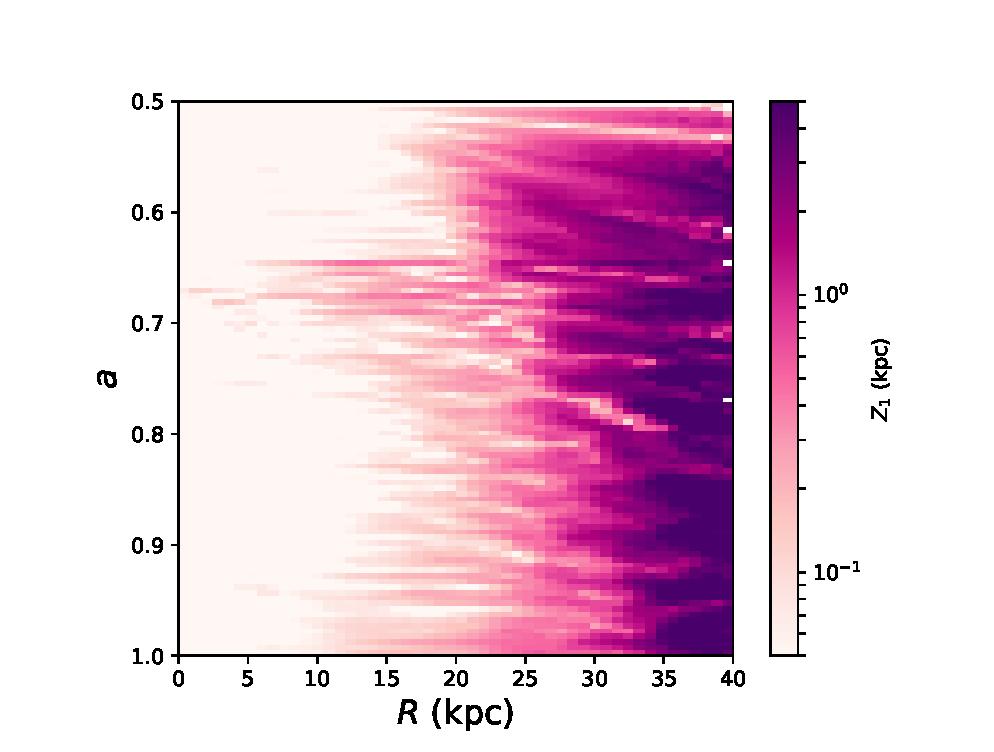
\includegraphics[width=0.45\textwidth]{../figures/c_early_z_1_r_a.eps} \label{fig:c_early_r_a_1}}\\
	\subfloat[]{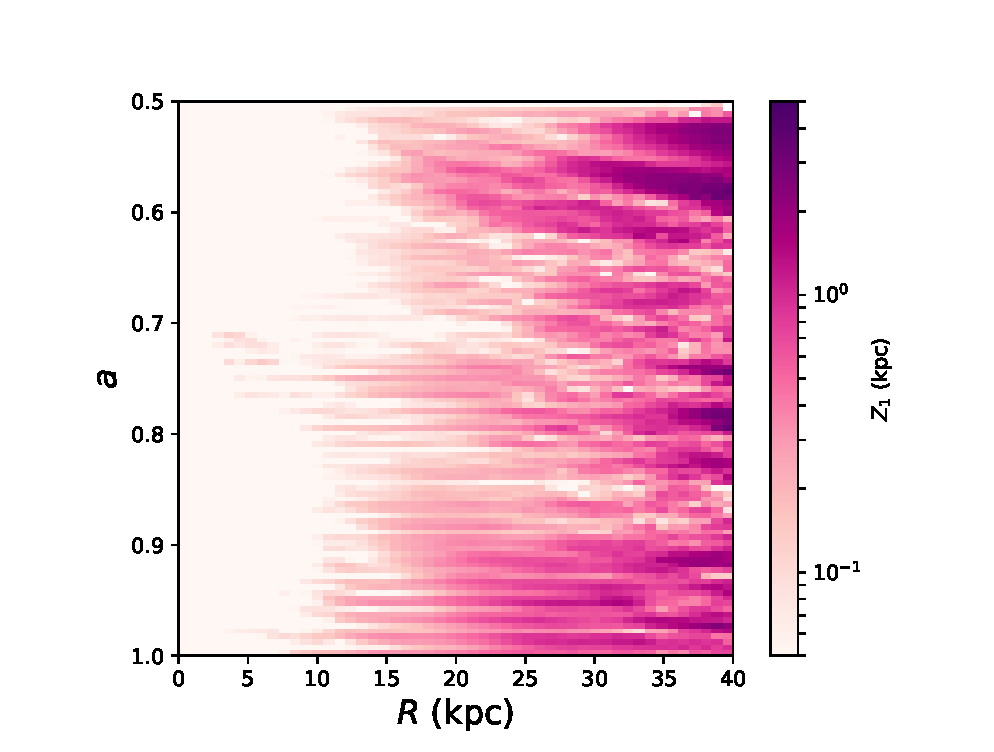
\includegraphics[width=0.45\textwidth]{../figures/a_early_z_1_r_a.eps} \label{fig:a_early_r_a_1}}	\caption{The $m=1$ bending mode for B.Late (a), C.Early (b), and A.Early (c) as a function of radius and scale factor. }
\end{figure}



Turning our attention to the longer term evolution of axisymmetric vertical structure in the disc, we study Fig. \ref{fig:b_late_r_a}. This figure corresponds to the mean height evolution of B.Late, our Sgr model. We can see an alternation of relative displacement of the outer disc as time progresses. The oscillations seen here are similar to the ones seen in the displaced disc experiment presented in \S\ref{ssec:toy_model_2}, which was loosely based on this simulation. Monoceros-scale fluctuations interior to 20 kpc occur almost instantly, and persist throughout the entire simulation. Interior to 15 kpc, the disc is quiet, much like the toy model. While there are some slight differences, we note the presence of another massive substructure in the the vicinity of the disc, so a one-to-one comparison is not expected.


In the case of pure misalignment, we look at the same plot for C.Early. Fig. \ref{fig:c_early_r_a} shows the evolution of the mean height as a function of radius and scale factor. We see the induction of corrugations on the scale of 100-200 pc as close in as $4\,R_d$ at early times. The inner disc on the other hand exhibits less of a signature from the uniform acceleration of the disc interior to 20 kpc than seen in B.Late. It is worth noting that the tidal arms generating the KUD stars in Fig. \ref{fig:xy_tidal_tail_halo_c} are reflected in the $m=0$ signature. At these large radii, we should see both the tidal arms which generate KUD stars and the tidal effect on the disc where present. In the case of C.Early, which is not substantially displaced as a result of substructure, this is entirely due to the grand-design spiral pattern created by misalignment from the host halo.

A more complicated scenario is presented by A.Early. Its displacement map is shown in Fig. \ref{fig:a_early_r_a}, and we immediately see very strong perturbations inside 20 kpc. These persist throughout the simulation, with the strongest perturbations being confined further out in the disc as the simulation progresses. A very interesting feature is the development of a net displacement of the disc center from the mean height. A displacement map for A.Early is shown in \ref{fig:a_early_displacement}. The central displacement appears to be a long-lived bending mode along the length of the bar, which we call a ``banana bar". 


In addition to flapping modes and axisymmetric displacements, we detect a strong $m=1$ warp signature in our three detailed examples. In the case of the pure satellite encounter, B.Late, we see a sub-kpc warp present in Fig. \ref{fig:b_late_r_a_1} during the first half of the simulation. As the substructure orbit continues, a close pass excites stronger $m=1$ structure. 

In contrast, the pure misalignment case, C.Early sees several kpc bending modes in the outer disc immediately. Furthermore, strong kpc-scale signal extends inside of 25 kpc at the beginning of the simulation where there is relatively little $m=0$ signature, and also where B.Late has relatively low $m=1$ signal. The contour of the $m=1$ bending mode post-buckling roughly traces the $m=0$ contour with a similar magnitude, suggesting a superposition of effects brought on by the environment's coupling to the buckling event.

The intermediate case, A.Early, presents something qualitatively between B.Late and C.Early. While the outer disc is initially excited, this extreme behaviour subsides as the halo equilibrates. Rather, we see a somewhat consistent, weaker several hundred pc signal in the inner and outer disc over the simulation. Lastly, buckling has a less drastic impact on the $m=1$ signature for A.Early than it did for the $m=0$.



\section{Discussion} \label{sec:discussion}

In this section, we compare the key points of our work to relevant literature. We find broad consistency across a variety of categories including disc flapping, bending, and stripping from the outer stellar disc.

\subsection{Disc Flapping}

Perhaps the most obscure effect we explored was the generation of flapping modes from inertial acceleration. \citet{sellwood_1996} presented the first in-depth study of this phenomenon in isolated galaxies. We find that the cosmological environment can generate the kinds of conditions that lead to substantial disc flapping. We see this happen in two key scenarios: when the inner disc-halo system is placed on a polar orbit with a distant, massive substructure, and when a bar buckles in an environment with high torque from the smooth halo. 

There is reason to think that the first of these scenarios is uncommon, or is at least secondary to other effects like bending. \citet{gomez_2017} ran MHD simulations where they note a lack of U-shaped warps, presumably caused by flapping. While these simulations contained many satellite mergers, the dominant effect in their simulations was an S-shaped warp. B.Late is a perfect example of a simulation where flapping modes can be seen as the dominant effect; it has no buckling bar and is initialized in a quiet halo. For both A.Early and C.Early, we would be hard pressed to say that we see the same kind of behaviour, especially where the disc is decently resolved.

The bar buckling generation mechanism for flapping modes is prominently displayed in C.Early. After the bar buckles, we see axisymmetric fluctuations in the mean height, as well as substantial flapping in the region of Monoceros. C.Early is clearly an outlier in this respect, and we suggest that bar buckling in conjunction with triaxility is a viable mechanism for corrugations in cosmological simulations. The general effect of bar buckling appears to introduce a signal in mean height, consistent with the simulation in \citet{bar_buckling_echo}. It may be possible to show that in general, disturbances from bar buckling are amplified in the presence of strong tides.

\subsection{$m=1$ Bending}



The $m=1$ signal appears to be the dominant mechanism in the outer disc in our simulations. Where we have substantial non-equilibrium activity, we see 100 pc scale activity that appears more ubiquitous than $m=0$ bending of that scale. Inspection of displacement maps at intermediate times reveals a picture consistent with the MHD simulations of \citet{gomez_2017}. The dominant state for the outer disc is some kind of S-shaped warp when it is present. 

Consistent with \citet{gomez_2017}, we find that halo misalignment is not a likely source of bending in the inner disc. Rather, most of the $m=0$ and $m=1$ in the inner disc appears to be associated with bar buckling. However, the outer disc is almost definitely affected by the smooth halo's tides. We see this in C.Early's $m=1$ profile being much stronger than either B.Late or A.Early in the outer disc.


Interactions with substructure also do not appear to show any signal in $m=1$ bending for the inner disc before buckling. There is, however, a strong $m=1$ signal in the outer disc in A.Early and B.Late. This roughly correlates with disc flapping. While the discrete pericentric passages do not appear in the $m=1$ signal, it appears that substructure is also effective at generating this kind of vertical structure in the outer disc.Once again, we infer that in the Milky Way, bar buckling would be the most likely culprit of $m=1$ bending in the solar neighborhood. B.Late, C.Early, and A.Early all show substantial signal in the solar neighborhood after bar buckling. Furthermore, like in the $m=0$ case, this appears long-lived. A.Early and C.Early both show strong $m=1$ signal for several Gyr after their bars buckle.


\subsection{KUD Stars and Feathers}

In terms of explaining how stars can be kicked to relatively high latitudes, we make progress here as well. \citet{laporte_2018_b} looked at several massive Sgr encounters ($8 \times 10^{10} \, \solarm$ and above) where the orbits pass right through the midplane. \citet{laporte_2018_b} and \citet{laporte_2019_feathers} found that in these mass regimes, stars could be kicked up to the latitudes consistent with our KUD population and low latitude Milky Way streams. 


Of course, the proposed mass in \citet{laporte_2018_b} is at the higher end of estimates for the mass of the Sgr dSph progenitor, and it isn't clear that less massive satellites can produce the same effect. The simulation, B.Late, demonstrates the potential issues of an Sgr dSph origin for KUD stars. As we saw in \S\ref{ssec:halo_env}, B.Late has a close encounter with a $3 \times 10^{10}$ substructure passing through the disc on a polar orbit around $a=0.885$. 

This passage follows substructure's passage through the disc plane at $a=0.875$. The orbit is similar to model L1 in \citet{laporte_2018_b}. Consistent with their findings, it does not appear that even this quite massive perturber can excite the kind of structure seen in other simulations in our suite. This can be seen in Fig. \ref{fig:lb_halo_b_late} at several heliocentric radii. We clearly see that the disc exhibits a corrugated structure, but that stars are only kicked up to $b<20^\circ$. 

We note that the simulations in which KUD stars reach their highest latitudes are the ones with substantial inner-halo-disc axis misalignment, namely C.Early and bauer2018b.Early. These are also the simulations with the highest $m=1$ bending signature in the outer disc. We address the question here of whether or not a distinct observational signature exists for a misalignment scenario versus simple substructure interaction. We understand this to be because in the absence of a very massive substructure, disc-halo misalignment is the only collisionless mechanism that can create strong enough $m=2$ perturbations for the mechanism suggested by \citet{laporte_2019_feathers} to act.

The big picture is that specific torques on the order $10^3 \, \kpc^2\,\text{Gyr}^{-2}$ are responsible for high latitude features. Kicking stars to higher latitudes either requires an extremely massive perturber, or substantial misalignment with the host halo. It is also possible that specific properties of the orbit may enhance the stripping mechanism, much like other resonant mechanisms in disc mechanics.

The global dynamical picture is consistent with the study presented by \citet{laporte_2019_feathers} that these perturbed stars remain close to each other in phase space. For instance, B.Late forms its KUD stars at two discrete times from narrow regions of the disc. By the end of the simulation, these stars still appear associated with each other in phase space. 

We can also infer from our simulations that for some mono-abundant chemical population at $z=1$, we would expect to see dynamically coherent (as supported by how stars are clustered by their kick-up time in the final snapshot) structures with a consistent chemical abundance. This is consistent with observations by \citet{bergemann_2018}, which found narrow abundance spreads for M-giants in A13 and TriAnd. The clustering of stars by their kickup time is true whether they were kicked by substructure, as in B.Late, or by the smooth halo, as in C.Early.



\section{Conclusions}

Our main findings can be summarized as follows:
\begin{itemize}
\item Final bar strength is qualitatively similar in all models regardless of environment.
\item Monoceros-like perturbations can form in a wide variety of cosmological environments, whereas higher latitude features appear more exclusive to environments with global tides.
\item Stars can be kicked out of galactic discs relatively easily and consistently through global tidal interactions.
\item The initial dynamical temperature of the disc modifies the resulting vertical structure, but does not suppress bulk vertical motions.
\item If a recent Sgr interaction is the cause of observed low-latitude streams, the progenitor mass is likely closer to $10^{11} \,\solarm$ than $10^{10} \,\solarm$.
\item A vertically asymmetric bar may be a unique signature of a cosmological environment with no global tides or close substructure encounters.
\item Bar buckling echos for many Gyr in a cosmological setting.
\end{itemize}

Simulations like these a treasure trove of information. We have presented the first step in analyzing the driving mechanics behind the kicked-up disc and the generation of vertical structure. By presenting the vertical evolution of Milky Way models in a variety of cosmological environments, we can begin to piece together which factors are at work in our Milky Way. By first understanding the halo environments, we were able to deduce qualitatively different behaviour in the vertical evolution of our simulations. Nearly all of the differences can be explained by the environment, and factors like radial velocity dispersion do little to change the evolution of disc vertical structure.

What struck us most about these simulations was initially that some stars could be kicked to very high latitudes. Our findings are consistent with the idea that a substructure less massive than the disc is unlikely to be responsible for even low latitude streams seen in the Milky Way. However, we have found that any sort of misalignment of the disc axis from the halo's short axis generates these populations quite easily.

In quieter merger environments like the Milky Way models we studied, the dominant cause of vertical structure in the solar neighborhood is bar buckling. Although  we see vertical perturbations extending to the inner disc in a variety of halo environments, it is quite apparent that bar buckling is the most effective in the region of the Gaia footprint.

Taking these together, we have presented two observationally notable results. The first is that if we can establish that the Milky Way is aligned with the halo short axis, it would imply that the Sgr dSph is in the vicinity of $10^{11}\,\solarm$. This would be necessary to explain observed disc stars at higher latitudes. The second is that we might be able to establish substructure as the main driving force for vertical structure in the Milky Way's outer disc if we are able to observe a banana shaped bar. Given our small sample size, this hypothesis requires further study.

Studies like this one are inherently limited to small sample sizes, and we should explore in greater detail the results presented here. Such a wide variety of cosmological environments exist, and ours are by no means exhaustive. However, we have established that haloes with massive perturbers or halo misalignment tend to yield qualitatively Milky Way-like vertical structure. The power of the technique we employ in this paper is that by using the same disc, we can unambiguously begin to make claims about the significance of various aspects of the cosmological environment. Looking at large scale hydrodynamical simulations for these effects may be a more informative approach as large unigrid simulations approach sufficient resolution. Studying a wider variety of environments will certainly address some of the issues left open by this work. 

\section*{Acknowledgements}
{LMW and JSB are supported by a Discovery Grant with the Natural
  Sciences and Engineering Research Council of Canada. JSB acknowledges the excellent
  supervision of LMW over the course of his Ph.D., and the sacrifice of many noble 
  coffee beans.}

%%%%%%%%%%%%%%%%%%%%%%%%%%%%%%%%%%%%%%%%%%%%%%%%%%

%%%%%%%%%%%%%%%%%%%% REFERENCES %%%%%%%%%%%%%%%%%%

% The best way to enter references is to use BibTeX:

\bibliographystyle{apalike}
\bibliography{bibliography_paper_iii.bib} % if your bibtex file is called example.bib


%%%%%%%%%%%%%%%%%%%%%%%%%%%%%%%%%%%%%%%%%%%%%%%%%%


